\chapter{Methodology}~\label{chapter-methodology}
\epigraph{Is there method in the madness?}{Anon (1964--on)}
\buzzwords{Empirical Studies, Theoretical Framework, Conceptual Framework, make assumptions explicit, methodological analysis using prior publications to identify a vocabulary - SE in practice, qualitative analysis,  the 1-2-3 of research design (question - evidence - method) ...}

\begin{wrapfigure}{R}{0.7\textwidth}
  \vspace{-0.75\intextsep}
  \begin{center}
    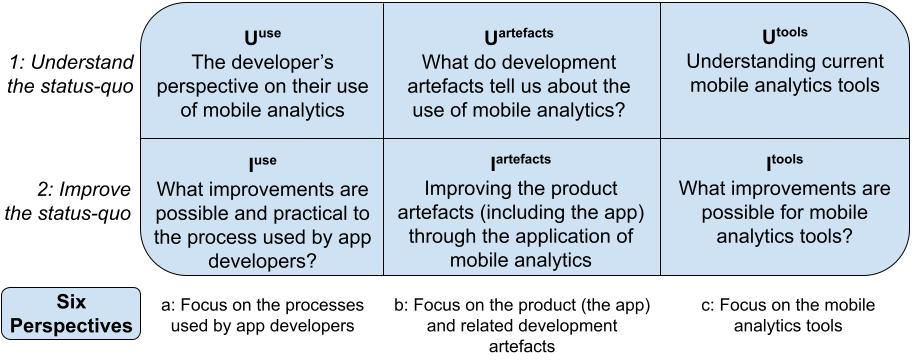
\includegraphics[width=0.66\textwidth]{images/my/six-perspectives-2x3-matrix-12-nov-2021.jpeg}
  \end{center}
    \caption{Methodology six perspectives (repeated)}
    \label{fig:six-perspectives-in-the-methodology}
\end{wrapfigure}

%In the Introduction (page~\pageref{rq-leads-to-six-perspectives}) six perspectives were introduced to support the main research question; these are repeated here in Figure~\ref{fig:six-perspectives-in-the-methodology} for ease of reference. These six perspectives consider three parallel topics: the processes, the products, and the mobile analytics tools in terms of the current practices - their use - and the scope to improve them.
%
%This research applies the 1-2-3 of research design (Question - Evidence - Method) which follow in the next three sections: 

The research needs to provide evidence to answer the main research question: \emph{How can applying analytics improve software development and software testing for mobile apps in practice?} (from Section \ref{overall-research-question}, page \pageref{overall-research-question}). The literature review has situated this question in existing research~\pending{do this once the Lit Review has been revised.}.  

To answer the research question the research needs to both understand the status-quo and to identify potential improvements, with respect to developer practices and thinking, apps and all the associated development artefacts (\textit{e.g.}, source code, issue tracking, tests, and operational configurations) that provide evidence of use, and the analytics tools themselves.

Improvements need to be compared to a baseline. In terms of this research the baseline has three perspectives: the processes currently being used by developers, the products of their development including the development artefacts and in particular the mobile app, and the mobile analytics tools themselves. Similarly it is appropriate to consider the improvements in terms of three perspectives, \textit{i.e.}: the processes, the artefacts including in particular the behaviour of the mobile app in use, and finally in terms of improvements possible in the mobile analytics tools. These are illustrated in the six perspectives introduced in the Introduction (page~\pageref{rq-leads-to-six-perspectives}) and repeated here in Figure~\ref{fig:six-perspectives-in-the-methodology} for ease of reference.

Therefore methodology needs to include techniques that can address these two key dimensions of investigation:
\begin{enumerate}
    \item a dimension that covers the different objects of analysis: the software development processes used by app developers; the software product (i.e. app) and related development artefacts; and the mobile analytics tools; 
    
    \item a temporal dimension that allows understanding of the current status and scope for improvements relating to the objects of analysis. It also needs to determine what \emph{is} and what \emph{could be}.
\end{enumerate}


\medskip

To describe the methodology chosen for this research, this chapter first identifies the evidence requirements in \secref{methodology-evidence-requirements}\improvement{I'm aware the first letter isn't capitalised of Section. I've got an action to improve the macro.} and then, in \secref{methodology-data-sources}, presents the data sources that were used, and then \autoref{methodology-methodology-section} describes the methodology used in this research. This is followed by \secref{section-introducing-the-case-studies}, which introduces two forms of case studies, those which are app-centric and those which are mobile analytics tool-centric, and the procedure used for app-centric case studies in \secref{methodology-app-centric-case-study-procedure}. The remaining sections cover the ethical aspects~\secref{methodology-ethical-considerations-section}, the threats to validity~\secref{methodology-threats-to-validity-section}, and finally a summary of this chapter in Section~\secref{methodology-summary-section}. 

\section{Evidence requirements}~\label{methodology-evidence-requirements}
Answering this research question requires rich, contextualised evidence of how developers use mobile analytics in practice.\pending{Add paragraph before this to replay findings of literature review, together with the overarching research question. If you organise your literature review as we discussed to use the three columns of the perspectives,  you could introduce the six perspectives at the end of the Lit Review. If the Lit Review takes a different direction introduce the six perspectives here.}  
Hence, the research needs to be situated in real-world industry practice and experience, drawing on real-world apps and projects for which analytics have relevance, \textit{i.e.}, that are part of an app-store ecosystem that collects analytics, and that are used by real-world users. The evidence needs to come from the developers, from their app microcosms, and from real-world mobile analytics.



% \newthought{The research needs to be situated in the real-world}
%As the real-world apps live in an app-store ecosystem, and as the main app stores collect app analytics, the research needs to be situated in apps that are available in an app store. And as the analytics are derived from usage the apps need to be used, ideally by real-world users of those apps. 

The goal of this research is to explore and understand the use and impact of analytics on mobile app development. %, rather than produce general findings that are applicable in all context.
Therefore, in order to gain an understanding of the six perspectives outlined in Figure~\ref{fig:six-perspectives-in-the-methodology}, it is necessary to investigate different examples of mobile app development practice. In this context, a comprehensive statistically representative sample of mobile apps was beyond the scope of a PhD, as determining the characteristics of sufficient representative apps and gaining access to their development contexts would be impractical. Instead, this research adopts the approach of `purposive sampling'  as described by ~\citep[pp180-182]{flick2018_an_introduction_to_qualitative_research_sixth_ed} as it was considered to be a more suitable approach. (Flick uses the term `purposive sampling' which is treated as a synonym of purposeful sampling in this thesis). A similar approach has been successfully applied by other researchers undertaking in-depth, qualitative explorations of software development practice, e.g., recent work on qualitative analysis of pair programming undertaken by ~\citep[p.114]{zieris2020_phd_qualitative_analysis_of_knowledge_transfer_in_pair_programming}\footnote{\emph{``Unlike for quantitative methods, statistical generalization from a sample to the population is not a goal. Instead, qualitative studies look for information-rich cases that allow to deepen the researcher’s understanding. Early in the process, each case is treated as unique and studied in great detail; cross-case analyses follow later and are based on the well-understood individual cases."}}. 

Flick presents six strategies of purposive sampling, in p.181. Of necessity the strategy used in this research is one described by Flick as convenience, however a more appropriate term for the strategy is opportunistic, since few of the case studies were convenient. As Flick notes wryly, on p.182, `the problem of access may be one of the crucial barriers' which particularly applies when seeking access to sensitive data and information about software failures for commercial mobile apps.

In terms of purposive sampling in the research I strove to use a variety of projects and apps including: commercial and volunteer led development teams, solo developer, small, medium and large development teams, industry and opensource apps, apps that include in-app mobile analytics and those that choose not to. Some of the projects that declined to participate in the research would have helped address some of the gaps in coverage of the known varieties of projects and apps.

The research explored a variety of analytics tools, as no two are identical: they offer a variety of features and capabilities, and have distinct behaviours.  Furthermore there are tools that work at the platform level and others that work at the app level; researching tools that work at both levels helps determine and distinguish their characteristics and compare their behaviours. There is only one platform-level mobile analytics tool in Google Play, the one that Google provides. In contrast there are tens of app level mobile analytics tools so there is value in researching several these app level mobile analytics tools.

The varieties of projects, apps, and mobile analytics tools, are all intended to help to uncover emergent features, capabilities, and behaviours; they also help establish ranges of examples of improvements and concerns. An additional objective is to increase the `weight of evidence' in support of particular propositions, rather than to prove them~\citep[see p.569]{seaman1999_qualitative_methods_in_esse}, which is impractical in the scope of this research.

Note: the collection of evidence depends on the source and the availability of that source in a particular study or context. It may also be constrained by technical, legal, logistical and other factors.

\section{Data sources}~\label{methodology-data-sources}
The nature of research in a sometimes messy real-world environment means access is opportunistic and often occasional. The evidence will be incomplete, yet rich, complex, and multi-faceted because of the variety of projects investigated in the research. For this research the data sources include:

\begin{itemize}
    \itemsep0em
    \item Development artefacts: their origin is the development team. They include: app binaries, app source code, tests, work schedules, documentation, bug tracking systems, \textit{etc.}, these were collected during the various case studies and complemented by public sources for additional mobile apps. 
    \item `Grey material': includes grey data and grey literature. Some were stimulated as part of the case studies, others were found during additional background research.
    \begin{itemize}
                \item Grey data includes: various discussion forums used by mobile app developers and other online contextual information, online issue tracking and related code for opensource projects beyond those that were the focus of the app-centric case studies developed in this research (e.g., open source networking libraries used by Android apps). 
                \item Grey literature includes: online materials on mobile analytics tools, articles including on medium.com and various blogs. Some were found in response to findings during particular case studies, others were found during additional background research.
    \end{itemize}
    \item Pre-study interviews: with developers and as appropriate authorised representatives of their organisation. These were used for setting up the study and understanding the development context. They were collected as part of the case studies.
    \item Mid-study communications with developers: usually email correspondence for clarification, to obtain updates, or comment on observations. These were collected as part of the case studies.
    \item Field notes: some handwritten, others recorded as text on computers. These were collected as part of the case studies and during background research.
    \item Analytics tools and associated analytics artefacts: their origin is the mobile analytics tool. Analytics artefacts, in particular, were a key data source; they include various outputs including screen captures, screen-scraping and parsing, results from calling APIs, and automated emails generated by analytics tools. Product documentation, online help materials, examples, and so on were also used as data sources. For open source analytics tools, the code was also used as a data source. All these data sources were collected on an ongoing basis during case studies and during additional background research.
\end{itemize}

The evidence is mainly based in real-world cases, augmented with micro-experiments where these were more appropriate. For all of these real-world cases, collection of naturally-occurring data (e.g., development artefacts, grey material) was augmented by elicitation of additional data (e.g., interviews and communications with developers) to provide clarification, breadth and insight.  Different research methods made use of these data sources, as appropriate.

In terms of the methodology, during the active case study it is vital to collect and perform ongoing analysis of mobile analytics and whatever other materials are available. Many of these are ephemeral in nature. For instance graphs generated by analytics tools may change by the minute. There is seldom a manual for the mobile analytics outputs (\textit{e.g.} the reports), furthermore many of the reports are dependent on the underlying data and/or on changes in the underlying service, Therefore the researcher often needs to iteratively learn the mobile analytics reporting in an exploratory manner\pending{Add a link to the Expo example from LocalHalo as an example}.


Third-party mobile analytics (including those provided by Google) have terms of use. These terms of use have various names, such as a policy, \textit{e.g.} for Google Play ~\citet{google_play_developer_policy_center}. These may place limitations on data collection and use of the relevant service. For the research covered in this thesis a conservative approach was used in terms of data collection to reduce the risk of consequential issues for the researcher, the project, and the stakeholders for the app. This topic and the implications are expanded on in the Discussion chapter in Section~\secref{discussion-considerations-on-the-method}, starting on page~\pageref{discussion-considerations-on-the-method}.

The choice of tools, including the humble web browser used by the researcher, affects aspects of the ease of collection of on line reports. As an example, the screenshot capability of the Mozilla Firefox browser~\footnote{Described in \url{https://screenshots.firefox.com/}} is far richer than that provided by Google Chrome at the time of writing. Many of the reports in mobile analytics tools require extensive vertical scrolling, Firefox can capture the entire contents easily, Chrome does not. 

Similarly some content is only generated on screen on demand, in response to user actions, for example through scrolling vertically (such as using `infinite scrolling'~\citep{parker2012_infinite_scrolling}) and/or paging through reports. Others are contextual and may only appear when the relevant conditions occur. For example, the release management reports in Google Play Console appear for the first 7 days of a new release. Therefore, to capture the content the researcher (or their human/automated proxy) needs to perform these actions to obtain these contents and pertinent materials saved/safeguarded to facilitate longer term analysis and provide/record evidence. Where practical, the underlying text was collected in addition to visual content; we created software called Vitals Scraper do so for Google Play Console with Android Vitals. The text could then be processed relatively easily and without needing to be re-keyed. Note: it is not always practical or useful to record ``everything"; how much is suitable is a topic for future research. 

\subsection{Mapping the data sources to the six perspectives}
The various data sources described in the previous section each contribute to the six perspectives as indicated in Table~\ref{tab:mapping-datasources-to-six-perspectives}. The table has two indications of the strength of the contribution: `\textbf{S}' indicates a strong contribution, and `\textbf{m}' indicates a moderate contribution. The blank cells indicate low, or marginal, contributions rather than necessarily no contribution at all.

\begin{table}
    \small
    \setlength{\tabcolsep}{4pt} %% default is 6pt
    \setlength{\arrayrulewidth}{0.1mm}
    \centering
    \begin{tabular}{l|ccc|ccc}
      & \multicolumn{3}{c|}{\bfseries \small Understand} & \multicolumn{3}{c}{\bfseries \small Improve} \\
      \toprule
         % &\textsubscript{u}Use &\textsubscript{u}Artefacts &\textsubscript{u}Tools &\textsubscript{i}Use &\textsubscript{i}Artefacts &\textsubscript{i}Tools \\
         \multicolumn{1}{r|}{Six perspectives} &\uuse &\uartefacts &\utools &\iuse &\iartefacts &\itools \\ % Thanks to https://tex.stackexchange.com/a/33488/88466
        \hline 
        Development artefacts                       &S &S &m &m &m &m \\
        Grey Data                                   &S &m &m &  &  &  \\
        Grey Literature                             &m &m &m &m &m &m \\
        Pre-study interviews                        &S &  &m &m &m &m \\
        Mid-study communications with developers    &m &m &m &m &m &m \\
        Field notes                                 &S &m &S &S &S &S \\
        Analytics tools \& artefacts                &m &m &S &m &S &S \\
        \bottomrule
    \end{tabular}
    \caption[Mapping data source (rows) to the 6 perspectives (columns)]{Mapping data source (rows) to the 6 perspectives (columns) \\ S = \textbf{S}trong contribution \\ m = \textbf{m}oderate contribution}
    \label{tab:mapping-datasources-to-six-perspectives}
\end{table}

Development artefacts contribute strongly to understanding of the use of mobile analytics and the artefacts themselves. They also contribute to the understanding of mobile analytics tools, for instance as they contain the usage of any API's provided by a mobile analytics tool. Through understanding the development artefacts various potential improvements emerge across the board for each of the three objects of analysis.

Grey data, \textit{e.g.} developer-centric discussions in project issues on GitHub and Q \& A on StackOverflow, mainly contribute to understanding the current state of affairs, both the immediate issues and historical issues that may or may not have been addressed or retired through changes to the mobile analytics tools and any of their associated SDKs. While they may also hint at future improvements that's seldom the focus of the developer-centric discussions. That said, occasionally external developers to a project may also suggest and/or contribute specific improvements.

Grey literature can contribute to all six perspectives moderately. It is unlikely to contribute strongly to any, partly as the material tends to be general in nature rather than specific to particular apps or projects.

Pre-study interviews mainly contribute to understanding a team's current use of mobile analytics tools. They seldom get into detail of the development artefacts, apart from various statistics that are reported by mobile analytics tools \textit{e.g.} the crash rate of the team's app(s). They often indicate areas of improvement across the board that the team could make, but not in enough detail to provide concrete improvements at this early stage in the relationship.

Mid-study communications are often focused on understanding immediate and recent events from a variety of sources (including use, changes to the artefacts, outputs from the mobile analytics). During discussions that are part of the communications scope for improvements emerge across the board.

Field notes may well be the strongest data source overall, the only area where they're limited to a moderate contribution is in terms of understanding the artefacts - generally the understanding of the artefacts is primarily evidenced in the development artefacts directly, so the field notes augment these rather than being the strongest source of information for \uartefacts.

Perhaps unsurprisingly, analytics tools and associated artefacts contribute most strongly to the use and improvement of the tools themselves. They also contribute strongly to improvements in the artefacts \textit{e.g.} through identifying areas in the source code that lead to a crash.


\section{Methodology}~\label{methodology-methodology-section}
The germs of the methodology include three primary complementary sources: Ball and Ormerod's `cognitive ethnography', Runeson and Höst's `guidelines for conducting and reporting case study research in software engineering', and Seaman's `Qualitative methods in empirical studies of software engineering'~\footnote{Note: this methodology was also influenced by additional research from a variety of authors in the fields of software engineering and \href{glossary-esse}{ESSE}.}.

Broadly, this research starts from what Ball and Ormerod described as `cognitive ethnography'~\citep{ball2000_putting_ethnography_to_work_cognitive_ethnography}, that is, observation-based enquiry conducted \textit{in situ} to investigate ``...the interplay between people-laden contexts and expert cognition'' (p. 149). Ball and Ormerod characterise cognitive ethnography in terms of observational specificity, verifiability and purposiveness: 

\begin{quote}
  \textit{``Our own conception of cognitive ethnography is characterized by three key features. First, it relies on small-scale data collection based around representative time slices of situated activity. As such, it demonstrates observational specificity, as opposed to the intensity of a prototypical ethnography. Second, it is purposive, in that its mode of questioning focuses on issues that are informed by some intention to intervene with, or somehow affect, existing work practices ... Third, it places a strong emphasis on verifiability, in terms of validating observations across observers, data sets and methodologies.''}   ~\citep[p.152]{ball2000_putting_ethnography_to_work_cognitive_ethnography} 
\end{quote} %

Consistent with this orientation, this research sought to derive a situated understanding of analytics (in terms of the six perspectives in Figure~\ref{fig:six-perspectives-in-the-methodology}). The insights that emerged from the more ethnographically-inspired analysis of naturally-occurring data were then investigated further and tested using other approaches, namely across-case comparison, hypothesis testing (systematic manipulation in micro experiments) and action research (evaluation through interventions in specific cases) -- consistent with Ball and Ormerod's emphasis on verifiability.  

As Runeson and Höst note, software engineering motivates specialised research methodologies as the study objects: develop software, they are project oriented, and the work is advanced engineering work by highly educated people~\citep[pp. 132-133]{runeson_2008_guidelines_for_conducting_and_reporting_case_study_research_in_sw_eng}. % See below comment for the relevant text.
These criteria apply to all the case studies in this research and therefore specialised research methods were developed in order to perform the research effectively and productively. 

\begin{comment}
The study objects are 1) private corporations or units of public agencies developing software rather than public agencies or private corporations using software systems; 2) project oriented rather than line or function oriented; and 3) the studied work is advanced engineering work conducted by highly educated people rather than routine work. 
\end{comment}

My research is situated in development teams who create mobile apps and use software tools - in particular mobile analytics - in order to provide apps that work adequately for their userbases. As Seaman notes, it's important to study \emph{``nontechnical issues and the intersection between the technical and nontechnical in software engineering"}~\citep[p.557]{seaman1999_qualitative_methods_in_esse}. The author further notes the key advantage of using qualitative methods is to force the researcher \emph{``to delve into the complexity of the problem rather than abstract it away."} (p.557).

\begin{figure}
    \centering
    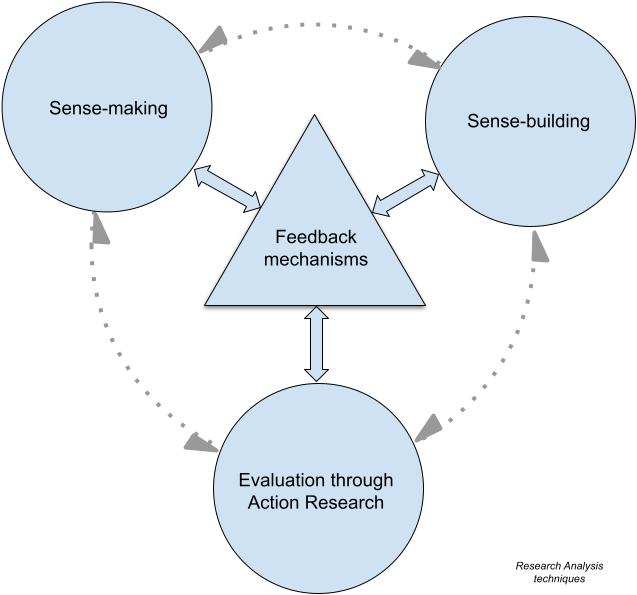
\includegraphics[width=10cm]{images/my/analysis-techniques-in-PhD-08-Nov-2021.jpeg}
    \caption{Categories of research methods}
    \label{fig:categories-of-research-methods}
\end{figure}

\subsection{Categories of research methods}
Figure~\ref{fig:categories-of-research-methods}, on page~\pageref{fig:categories-of-research-methods}, provides a visual overview of the four categories of research methods used to serve this `cognitive ethnography' approach; they include 1) sense-making, 2) sense-building, and 3) evaluation through action research. These were complemented by the fourth category 4) feedback mechanisms to help support and verify the analyses. 

Note: Figure~\ref{fig:categories-of-research-methods} is an over-simplification with clear boundaries between the categories in order to convey the alignment of methods to purposes, and the categories are not discrete.  Some methods include several data sources, and some data sources are analysed using several methods. In practice, individual research methods provided multi-faceted contributions; for instance local app experiments contributed to both sense-building and sense-making. 


\medskip

Table ~\ref{tab:mapping-analysis-to-six-perspectives} identifies the various research methods, groups them in terms of their roles in the research (as illustrated in Figure~\ref{fig:categories-of-research-methods}), and maps them to the six perspectives.  Each of these research methods includes data collection \textit{and} analysis unless otherwise stated.


\begin{table}
    \small
    \setlength{\tabcolsep}{4pt} %% default is 6pt
    \setlength{\arrayrulewidth}{0.1mm}
    \centering
    \begin{tabular}{l|ccc|ccc}
      & \multicolumn{3}{c|}{\bfseries \small Understand} & \multicolumn{3}{c}{\bfseries \small Improve} \\
      \toprule
         % &\textsubscript{u}Use &\textsubscript{u}Artefacts &\textsubscript{u}Tools &\textsubscript{i}Use &\textsubscript{i}Artefacts &\textsubscript{i}Tools \\
         \multicolumn{1}{r|}{Six perspectives} &\uuse &\uartefacts &\utools &\iuse &\iartefacts &\itools \\ % Thanks to https://tex.stackexchange.com/a/33488/88466
         
        \hline 
        \textbf{Sense-making} & & & & & & \\
        (comprehension and exploration) & & & & & & \\
        Beacon finding and    &S &m &S &m &m &m \\
        Drill Down            &m &m &S &S &m &m \\
        %\tabucline[1pt on 3pt]  \\ % See https://tex.stackexchange.com/a/109301/88466 however here it is terminated prematurely and a bit heavy 
        % Or try https://tex.stackexchange.com/a/229334/88466 or https://tex.stackexchange.com/a/613907/88466 if I've not collapsed these two previous rows soon.
        % Or use a newer latex package, see https://tex.stackexchange.com/a/611494/88466 

        \hline
        \textbf{Sense-building} & & & & & & \\      
        %(Integration and differentiation)    & & & & & & \\        
        (micro-experiments and macro-discoveries) & & & & & & \\
        Local App Experiments   &m &S &S &  &S &S \\
        FOSS Contributions      &  &  &S &  &  &S \\
        Across Case Comparisons &S &m &S &S &m &m \\        
        
        \hline
        \textbf{Feedback mechanisms} & & & & & & \\
        (triangulation and validation) & & & & & & \\
        Ask The App Devs      &S &m &m &m &m &m \\
        Ask The Tool Devs     &  &  &S &m &m &m \\
        Grey Literature \& Grey Data Analysis       &m &m &S &m &m &  \\
        Code, \& app-binary, Analysis         &m &S &  &m &m &  \\
                
        \hline
        \textbf{Evaluation through action research} & & & & & & \\
        (embedded intervention)  & & & & & &  \\
        Observation and Analysis &S &S &S &S &S &m \\
        Field Experiment         &m &  &  &S &S &  \\
        Hackathon                &m &m &  &S &S &  \\
        
        \bottomrule
    \end{tabular}
    \caption[Mapping research methods (rows) to the 6 perspectives (columns)]{Mapping research methods (rows) to the 6 perspectives (columns) \\ S = \textbf{S}trong contribution \\ m = \textbf{m}oderate contribution \\FOSS = Free and Open Source Software}
    \label{tab:mapping-analysis-to-six-perspectives}
\end{table}
\unsure{The "Yy" markers are inconsistent with "Sm" markers used in Table 1.1}

`\textbf{Sense-making}' methods were concerned with understanding current practice (as reflected in artefacts, tools, and developers' practices and perspectives -- i.e., perspectives \uartefacts, \utools, and \uuse) and identifying potential improvements in tools and in how analytics are used in app development and maintenance (i.e., perspectives \itools and \iartefacts). The research methods include beacon-finding (see page~\pageref{section-beacon-finding-method}) and drill-down (see page~\pageref{drill-down-research-method}).

Sense-making incorporates an iterative pattern of \textbf{beacon finding} to identify areas of interest within a case, \textbf{drill down}\unsure{Does putting the methods in bold help with readability?} to investigate one or more beacons, and comparisons both within and across~\footnote{While across case comparisons are grouped under sense-building they also help with sense-making.} cases to identify patterns, relationships, counterfactuals~\footnote{\emph{``...relating to or expressing what has not happened or is not the case." Oxford Languages.}}, as some characteristics emerge in contrasts across and between a body of studies. 
%
Comparisons were performed iteratively on an ongoing basis (for active apps the values are not constant). These comparisons included comparisons across releases, using different windows of time, on different dates, comparisons with peers, and so on.


`\textbf{Sense-building}' methods build on insights found through sense-making. The research methods included micro-experiments, carried out on local apps (see page~\pageref{local-app-experiments-research-method}), FOSS contributions\unsure{Arosha's suggested alternative concepts of white and black box testing of the tools. I'm mulling these over. TBD.} (see page~\pageref{foss-contributions-research-methods}), and across case comparisons (see page~\pageref{across-case-comparisons-research-method}).

Local app experiments (see page~\pageref{local-app-experiments-research-method}) were used to investigate detail and give insight into the relationships between tools, quality of analytics, and potential impact of analytics use on apps (i.e., perspectives \uartefacts, \utools, \iartefacts, \itools).

Across-case comparisons (see page~\pageref{across-case-comparisons-research-method}) identify macro-discoveries -- that is, they identify characteristics and patterns that were not evident in individual case studies, potential improvements to practice (i.e., perspectives \uuse and \iuse), as well as the influence of the quality of tools in practice (\itools). They can also corroborate and/or challenge findings found in individual cases.


`\textbf{Feedback mechanisms}' were used to support and verify the other analyses, by comparing observations to other evidence, or by asking developers for clarifications or reflections. Feedback mechanisms are used throughout the research and mainly contributed to the understanding of perspectives associated with (\uuse, \uartefacts, and \utools), nonetheless they were also frequently used when considering improvements (\iuse, \iartefacts, and \itools). 

`\textbf{Evaluation through action research}' methods were largely concerned with evaluation of the effect of improvements in the use of analytics, in terms of adoption into use and app performance (i.e., perspectives \iuse and \iartefacts). It includes three research methods: 1) observation and analysis, 2) field experiment, and 3) hackathon. These are explained in page \pageref{section-evaluation-through-action-research-method} onwards. 

The research was iterative, moving through sensemaking, sensebuilding and feedback mechanisms repeatedly as new cases are studied or new insights emerge.  The methods and the data sources often also inform several of the six perspectives.  These research methods are introduced in more detail in the sections that follow.

\subsection{Sensemaking}
% c.f. https://en.wikipedia.org/wiki/Sensemaking_(information_science)
%1) Identifying patterns (inductive analysis) c.f. grounded theory. 2) 

`Sensemaking' includes 1) beacon finding and 2) drill down. These were used for \textit{inductive analysis} of artefacts, broadly consistent with grounded theory where the statements or propositions are supported in many ways by the data discovered in development and analytics artefacts; \textit{c.f.} the discussion of `grounded theory' methods where the propositions are ``grounded" in the data~\citep[p.566]{seaman1999_qualitative_methods_in_esse}~\footnote{This research in turn cites:  Glaser, Barney G., Anselm L. Strauss, and Elizabeth Strutzel. \emph{"The discovery of grounded theory; strategies for qualitative research."} Nursing research 17, no. 4 (1968): 364., which I have not been able to access.}\pending{Marian to help with the grounded theory aspects e.g. via~\citep{zieris2020_phd_qualitative_analysis_of_knowledge_transfer_in_pair_programming}}. 

\julian{\textit{c.f.} `Cognition in the wild', as a comparison with grounded theory. Cognition in the wild provides a parallel example of rich and emergent findings from the real world that would be very hard to specify or determine the factors that applied at the time the ship was being brought under control~\citep{hutchins1995_cognition_in_the_wild}.}\pending{I'm waiting to borrow Marian's copy of this book, then I can write about the connection to this research and the methodology.}

These sense-making methods were amplified through the feedback mechanisms, covered shortly. 
%In addition a third method, local app experiments, was used to create conditions for additional sensemaking.

\begin{figure}
    \centering
    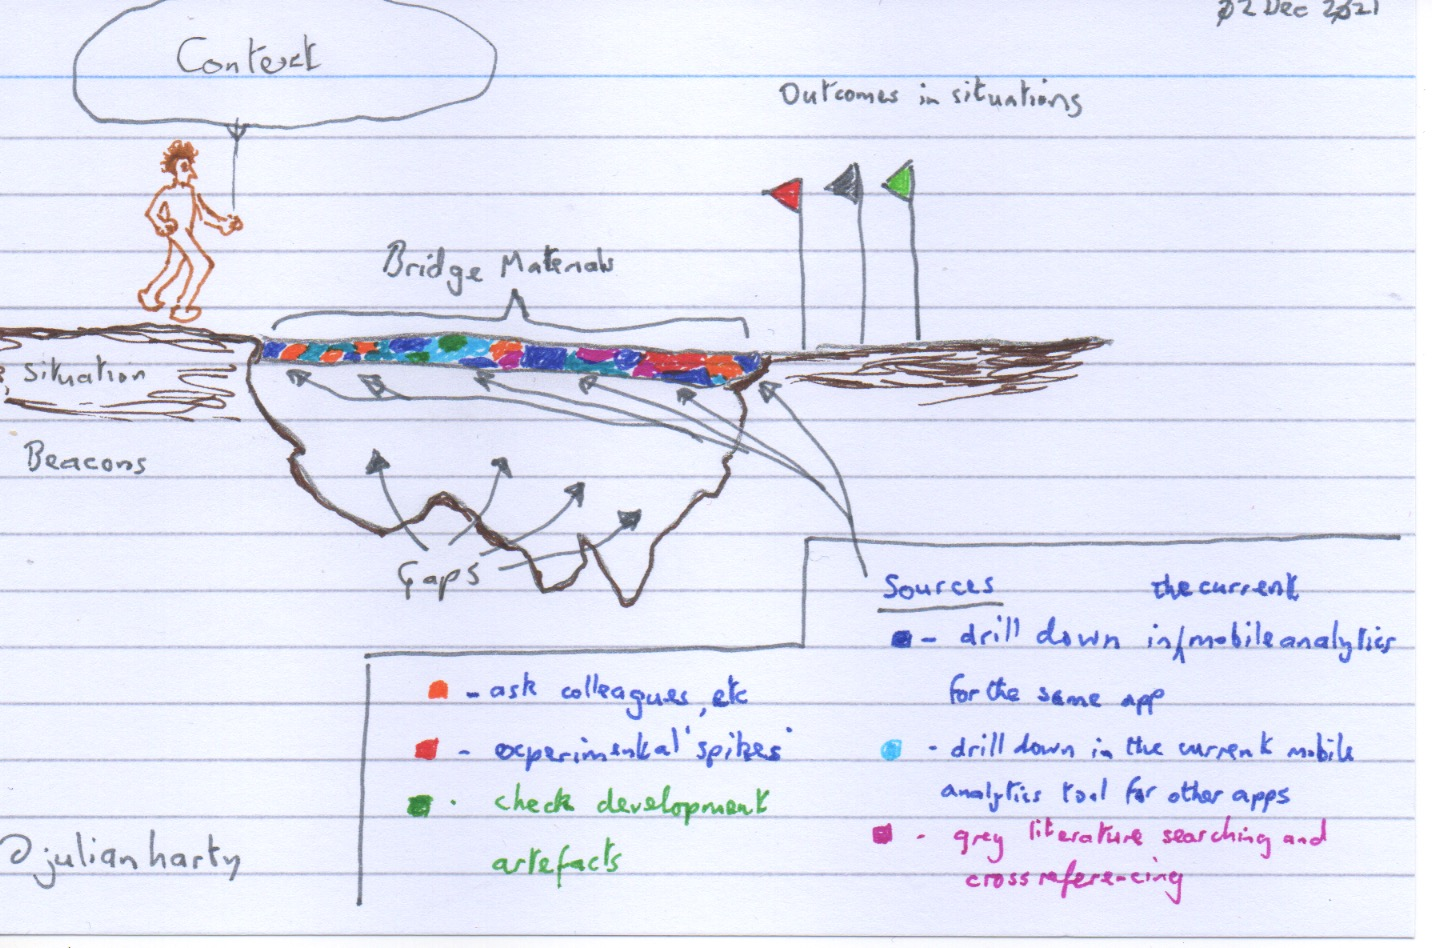
\includegraphics[width=15cm]{images/rough-sketches/the-sense-making-metafor-revised.jpeg}
    \caption{Custom Sense-Making Metaphor diagram}
    \label{fig:the-sense-making-metafor-revised}
\end{figure}

Sense-making has been used in research in Information Science, the topic is well summarised in \citealt{naumer2008_sense_making} co-authored by Karen E. Fisher, and by Brenda Dervin who created the sense-making methodology presented in this paper.\change{Change focus of this para. to sense-making rather than focusing on the authors.} Figure~\ref{fig:the-sense-making-metafor-revised} presents a revised edition of the Sense-Making Metaphor in Brenda Dervin's methodology adapted here to illustrate sense-making in this research. It broadens the approach to indicate the range of potential sources used in sense-making for mobile analytics, here illustrated with individual colours~\footnote{The choice and selection of colours illustrative and not intended to be definitive.}. The range of sources include:

\begin{figure}
    \centering
    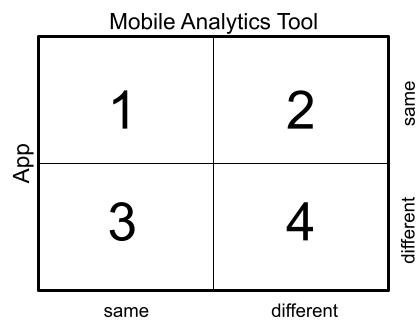
\includegraphics[width=6cm]{images/my/Boston-matrix-app-and-mobile-analytics-tool.jpeg}
    \caption{Boston matrix for app and mobile analytics tool}
    \label{fig:boston-matrix-app-and-mobile-analytics-tool}
\end{figure}

\begin{itemize}
\itemsep0em
    \item Drill-down (described in \secref{drill-down-research-method}) in the current mobile analytics tool for the same app (segment 1 in Figure~\ref{fig:boston-matrix-app-and-mobile-analytics-tool}).
    \item Drill-down in the current mobile tool for other apps (segment 3 in Figure~\ref{fig:boston-matrix-app-and-mobile-analytics-tool}). \\ (If the app incorporates other mobile analytics tools these tools may also help where there is overlapping content common to both tools; for example crashes reported in both Android Vitals and in Crashlytics, (segment 2 in Figure~\ref{fig:boston-matrix-app-and-mobile-analytics-tool}).)
    \item Comparing various analytics artefacts, particularly reports, using various criteria.
    \item Searching grey data and grey literature and cross referencing of materials.
    \item Asking people: for instance colleagues, the developers of the app, the developers of the mobile analytics tool, \textit{etc}.
    \item Experimental `spikes' where a simple,  minimal effort piece of code is written to try out an idea~\footnote{\url{https://en.wikipedia.org/wiki/Spike_(software_development)}}. (These tend to require significant effort so are not likely to be used lightly).
    \item Check development artefacts as these may provide relevant and pertinent information and clues.
\end{itemize}

In short, beacons need to be understood in context and the context includes seeking and obtaining additional information from a wide variety of sources. That said, of the many potential sources, two are core to sense-making: beacons are first found and thereby they also become a source and then drill-down used to make sense of the information pertaining to the beacon. The others are also useful, however for the purposes of this research they mainly serve another category and are therefore allocated to that category.

%Further reading: two of Brenda Dervin's figures for her sense-making metaphor are adapted very slightly if at all in https://asistdl.onlinelibrary.wiley.com/doi/epdf/10.1002/asi.20400 which focuses on gap-building~\citep{savolainen2006_information_use_as_gap_bridging_the_viewpoint_of_sensemaking_methodology}.

%Sensemaking has been applied to various aspects of computing and software development, for example: in program comprehension, in understanding end-users' understanding of spreadsheets~\citep{grigoreanu2012_end_user_debugging_strategies_a_sensemaking_perspective}. COULD-DO discuss the work of~\citep{naumer2008_sense_making}. Our use of sensemaking is inspired by sensemaking in research into these areas. 

%The following methods primarily helped with sense-making: analysing and ``making sense" of mobile analytics tools, development artefacts, and the developers' perspectives on their use of mobile analytics. 

\subsubsection{Beacon-finding}~\label{section-beacon-finding-method} %concept, adaption to suit this research, examples.

The notion of \textbf{`beacons'} is borrowed from research on program comprehension; for instance by Wiedenbeck, who helped establish the notion of beacons in software development: ~\emph{``In programming, beacons are lines of code which serve as typical indicators of a particular structure or operation"}~\citep[p.679]{WIEDENBECK1986_beacons_in_computer_program_comprehension}. The work was extended and updated to explicitly consider the effects of beacons in comprehension of source code, for instance in~\citealt{crosby2002_roles_beacons_play_in_comprehension_etc}.

The notion of beacons was generalised for this research to include indicators in the analytics of something of interest, or something that required attention.  And so 'beacon finding' was an inductive process by which significant indicators in the analytics data were used to identify areas of the code base that required further investigation.  Mobile analytics may include source code that calls APIs in the application's source code, however the bulk of the contents that need to be comprehended comes as outputs from the mobile analytics tools, therefore the beacons will differ accordingly. In this research the beacons include: the shape of graphs in mobile analytics report, failure clusters, a method call in stack traces, and so on\pending{I'm assembling some relevant raw notes in a new file: beacons-in-mobile-analytics.tex TBD where and how I'll integrate it.}.

%\marian{Now specify how you spotted beacons... I looked for things on this basis, how I kept track of things, what selection criteria were used and why?}

Beacons emerge in various ways. For instance in reports they include: anomalies within a report, mismatches and inconsistencies between two sibling reports or between a master report and the linked detailed report~\pending{Arosha, suggested introducing these terms for different types of report when discussing analytics tools in the lit. review. I agree, TBD once the lit. review has been reworked.}, in the shape of the curve of a graph, in the distribution and groupings of aggregate data, and so on. Similarly, alerts as determined by a mobile analytics service may be considered potential beacons being `promoted' by the mobile analytics reports. 

The most common method of recording potential beacons was using web browser screenshots and/or other mechanisms that preserved information electronically. Some were annotated as part of the beacon-finding and drill-down analysis. Additional notes were written both electronically and/or in physical notebooks. 

Selection criteria included: top ranking results, atypical rates of change, adverse changes to reliability, novel failures particularly for the most recent release, etc. A consistent and overriding criterion was to seek beacons that indicated flaws and failures that could materially and adversely affect the user experience of the app for one or more users of the app.


%\textbf{Beacon finding} seeks potentially relevant indicators, typically within bounded domain such as software code. Beacons help to convey meaning and are used for comprehension, for instance by programmers who wish to understand source code~\citep[page i]{crosby2002_roles_beacons_play_in_comprehension_etc}. The concept of beacons in source code has been studied by various authors for several decades; for instance by Wiedenbeck, who helped establish beacons in software development: ~\emph{``In programming, beacons are lines of code which serve as typical indicators of a particular structure or operation"}~\citep[p.679]{WIEDENBECK1986_beacons_in_computer_program_comprehension}. The work was extended and updated to explicitly consider the effects of beacons in comprehension of source code, for instance in~\citealt{crosby2002_roles_beacons_play_in_comprehension_etc}.
 


% I'm not sure where to discuss beacons in conversations: for instance in a developer's description of their use of mobile analytics to assess the quality of the app - they exist to me - TBD.


\subsubsection{Drill-down}~\label{drill-down-research-method}
Beacons stimulate interest; the interest needs to be satisfied one way or another by investigating the beacons and their underlying information sources. 
For example:  Are the identified beacons genuinely significant? What do they signify or relate to in the app and its usage, etc.?  Drill-down starts with the original data sources, but may draw in other data sources (such as the feedback mechanisms) for example to clarify relationships, responses by the developers, etc.

Here are 2 examples:  % Temporarily these are a list, they'll probably be embedded in the paragraph once the relevant examples have been incorporated. The pending command links were poorly formatted when the text was inline.
\begin{enumerate}
    \itemsep0em
    \item 1) investigating a large spike in the overall crash rate to determine the constituent causes \pending{Add link to an actual example in a case study}
    \item 2) understanding a Java WebView Exception \pending{Again provide a link to the example in my thesis)}.
\end{enumerate}

Note: it transpires developers use a similar form of sense-making, this is discussed in \secref{sensemaking-and-decision-taking-by-developers-section}, starting on page \pageref{sensemaking-and-decision-taking-by-developers-section}.

\clearpage
\subsection{Testing mobile analytics tools on a continuum}~\label{section-testing-mobile-analytics-tools-on-a-continuum}

\buzzwords{Translucence, various levels of opacity, white+grey+white box testing}

 The research includes three methods of testing in order to evaluate aspects of the mobile analytics tools.\improvement{FYI this subsection is a w-i-p to explore whether the following material is clearer and more faithful to the research than the current local app experiments and FOSS contributions. If it is, this section will be woven into the rest of the methodology chapter. The catalyst was a suggestion by Arosha on \nth{8} Dec 2021.} 
 They are all forms of micro-experiment. The methods of testing are loosely based on familiar concepts of black-box, white-box, and grey-box testing where there are various levels, or depths, of opacity in the system under test.

The tests include: testing the developer support channels, testing the process and experience of providing contributions to several opensource projects owned by mobile analytics tool providers, and testing mobile analytics tools by treating them as a black-box system under test (SUT) though the development of several small-scale Android apps. These small-scale apps were used to exercise the app store's pre-launch facilities and several of the in-app mobile analytics tools.\pending{This needs connecting to the material that follows.} 

Add a table: mapping the methods to the granularity, show the connection to the colour of box and how they connect to the object of the testing.\pending{Add a table showing the mapping}


\newthought{Developer support channels}


\newthought{Mini, local app experiments} 
Essentially the same story as it the local app experiments method.

\newthought{Testing contribution processes} 
Code contributions to opensource packages of commercial mobile analytics projects.
%
Essentially the same material as in the FOSS contributions method. The hypothesis was that some companies make their proprietary code available as opensource but do not actually accept contributions. The experiments involved creating small improvements to one or two aspects of their opensource projects and then creating pull requests to discover their acceptance process and what the results would be in terms of them accepting the pull requests.

\newthought{Working with the Iteratively product}
This experiment emerged from earlier collaborations with the founders of Iteratively. They offered free access to their product. The experiment incorporated their product into a small Android app where the analytics was routed by their SDK to Amplitude. The experiment provided a translucent view into their SDK and its behaviour in terms of the integration with Amplitude and also the support for custom implementations.

\newthought{Collaboration with Google is also a form of testing}
In some ways the collaboration with Google's engineering team was a form of testing to see whether they would firstly accept the contributions as valid and of merit, and then whether they would improve their product to address flaws reported to them during the collaboration. Google... TBC.

%%%%%%%%%%%%%%%%%% See also %%%%%%%%%%%%%%%%%%%%%%
% https://en.wikipedia.org/wiki/Transparency_meter
% https://en.wikipedia.org/wiki/Opacity_(optics)
\clearpage

\subsection{Sense-building}
Sense-building moves beyond sense-making. Sense-making aims to understand \textit{what is}, while sense-building extends sense-making with direct action and more active research, for instance: to devise and run experiments to learn more about the behaviours of mobile analytics, and to seek patterns and generalisations across tools, and case studies. Two methods were used primarily in sense-building -- local app experiments and across-case comparisons -- together with a third method, \href{glossary-FOSS}{FOSS} contributions. 

\subsubsection{Local-app experiments}~\label{local-app-experiments-research-method} 
\textbf{Local app experiments} were used to \textit{test the understanding} of the relationships between the usage and the analytics through manipulations of apps and observation of the effects -- hence, the local app experiments were used to test some of the patterns identified in the inductive analysis. They consist of \textit{micro-experiments} involved creating and developing small mobile apps intended to exercise particular aspects of mobile analytics~\footnote{Similar to the `invent the future' adage, for example: \url{https://quoteinvestigator.com/2012/09/27/invent-the-future/}}). The inputs to an app were directed in order to determine the outputs from mobile analytics. These helped to answer questions and gaps observed as part of sensemaking.  The local app experiments gave insight into the relationships between tools, quality of analytics, and potential impact of analytics use on apps (i.e., perspectives \uartefacts, \utools, \iartefacts, \itools). 

The apps that were developed as local-app experiments are small mobile apps and not intended for production use. They were developed in order to investigate the relationships between the inputs (such as usage) and the analytics outputs (such as reports) through deliberate manipulation of the inputs and observation of the consequences.  

The local-app experiments allow for tighter control on the usage, \textit{i.e.} the inputs, in comparison to the unfettered use of real-world mobile apps. They can help surface behaviours and provide for tighter evaluation in the early, pre-launch/pre-production phases. %I can't say feedback as that'd conflate the other use of feedback here in the methodology.
The local app experiments were used to test some of the patterns identified in the inductive `sensemaking' analysis.

Where practical the source code of these apps is made available under a permissive opensource license to facilitate further research by others and in order to facilitate inspection by and feedback from others.

%\akb{Also explain how the results of these experiments connected to other parts of the method? e.g., did they change / add to the sense-making activities?}
The results of the local app experiments helped augment the across-case experiments, particularly in terms of providing additional results to compare with those from the app case studies. They also informed discussions with the app and tool developers. 

\subsubsection{FOSS contributions}~\label{foss-contributions-research-methods}
\href{glossary-FOSS}{FOSS} contributions provided experimental evidence where contributions were offered to public repositories of opensource mobile analytics components to explore the repository's willingness to accept contributions and its process for doing so. The contributions were each intended to improve one or more elements of the respective codebase and thereby improve the respective product offering. They were small in size and made on an \emph{ad-hoc} rather than a systematic~\footnote{While systematic contributions may be a valid approach to research this topic, it was not core to this research.} basis.


\subsubsection{Across-case comparisons}~\label{across-case-comparisons-research-method}
\textit{Across-case comparisons} were concerned largely with understanding current practice and identifying potential improvements to practice (i.e., perspectives \uuse and \iuse), as well as the influence of the quality of tools in practice (\itools). This method draws on the approach discussed in \citet[pp. 567-569]{seaman1999_qualitative_methods_in_esse}, \textit{e.g.} to compare pairs of case studies to determine variations and similarities, with the additional considerations of seeking areas of potential improvements based on findings from the various case studies.

Similar to using various software testing techniques to find bugs, making comparisons across the case studies can help to identify more of the behaviours of mobile analytics, their use, and their efficacy. Across-case comparisons can increase the probability of seeing fresh characteristics and establish similarities across cases. The comparisons across case studies help establish norms (which can also be used to identify beacons, and anomalies), patterns (and anti-patterns), variety, and ranges. 

Comparisons across cases (\textit{i.e.} across projects and their mobile apps) helps both researchers and developers, albeit their interests and focus may differ.

\begin{itemize}
    \item \textbf{For developers}: they can compare the reports for their apps with the results others obtain. Doing so may help them identify problems-in-common (shared problems) and fixes-in-common that work for many apps with similar failures. They can also establish norms and the comparisons help provide triangulation and perspective. Some developers also find peer-group comparisons stimulating.
    
    \item \textbf{For researchers}: across case comparisons include `plus one'~\citep[pp 28-29]{aurini2016_how_to_of_qualitative_research} research that can help uncover emergent behaviour, reinforce existing findings, and so on. The across case comparisons also provide additional microcosms where new findings are discovered in the behaviours of apps, the tools, the development practices, and the efficacy of the use of mobile analytics performed by a wider variety of development teams.
\end{itemize}


The data and the system state for individual apps can help to increase the `coverage criteria' for a mobile analytics tool (which may be considered a system or simply a `box' as in black-box, grey-box, or white-box system)~\pending{In the planned Tools chapter I can discuss this property of the various Mobile Analytics tools.}. 

We know from a related domain, software testing, that more test cases can increase the detection rate of behaviours. For example, a paper by~\citet{briand2007_a_critical_analysis_of_empirical_research_in_software_testing} discusses concepts including the concept of a cost-effectiveness curve and of what the author terms `random variations' and the effect these random variations have on fault detection effectiveness in page 5 of their paper. The set of inputs (\textit{e.g.} crash reports) into mobile analytics tool may result in various beacons - and related data - appearing in the outputs. By increasing the sets of inputs, particularly from dissimilar apps, there is the potential to increase the appearance of more beacons. And the larger volume of beacons across the projects allows for weightier analysis.

A key observation is that detection is not static nor a one-off value; behaviours come and go, particularly in mobile analytics tools where reports are often ephemeral. The value of across-case comparisons increases when the sampling increases to record more of the ephemeral behaviours and outputs.

The nature of this PhD research based on a relatively small number of apps and associated case studies means it is premature to attempt to systematically plot the number of cases against the behaviours that were observed. Instead the focus is on monitoring 
new insights vs. resonance, and how often a new case highlights something that was not noticed in previous ones, even though they were there~\footnote{\textit{c.f.} Testing and Noticing~\citep{bolton2009_testing_and_noticing} which discusses noticing (and not noticing) from a software testing perspective.}.

We also need to consider: does anything generalise beyond a single case?   


\subsection{Feedback mechanisms}
Sense-making and sense-building methods are centred on the research and driven by the researcher's focus and perspective. Unaided -- even if they are productive -- they risk being marginalised and disconnected from the work of others, in particular the work of those who actually develop the apps and the tools. 

This research used four `feedback mechanisms' to validate and challenge the research outputs of sense-making and sense-building:
\begin{itemize}
\itemsep0em
\item ask the app developers
\item ask the tool developers
\item analysis of grey literature and grey data
\item analysis of code
\end{itemize}
The first two (i.e., the mid-study communications with developers) extend understanding of topics emerging from sense-making or sense-building, consistent with Ball and Ormerod's `cognitive ethnography'~\citep{ball2000_putting_ethnography_to_work_cognitive_ethnography} and Petre's `targeted observation'~\citep[p.234]{petre2009_insights_from_expert_software_design_practice}, by engaging with the developers who are situated in their actual practice in their real-world microcosm.  For example, the developers can be asked about their experiences, perceptions or reasoning about emergent observations, or to explain particular decisions or practices that have been highlighted by the research. The latter two feedback mechanisms provide comparison to additional data drawn from analysis of existing information (i.e., grey literature, grey data, code).  The feedback mechanisms draw on multiple data sources, including some which are independent of the research, hence allowing for comparison/triangulation/colligation -- all with a focus on the research questions.


% \phantomsection
\label{method-vectored-questions}
%A method termed `\textbf{vectored analysis}' was used with both app developers and and analytics tool developers, \textit{i.e.} during two of the feedback methods: 1) ask the app devs, and 2) ask the tool devs. 
%Vectored observations/questioning/analysis was used with the aim of increasing the understanding of their work pertaining to mobile analytics. Vectored questions are purposeful and focused, they are similar to Petre's `targeted observation'~\citep[p.234]{petre2009_insights_from_expert_software_design_practice} and situated in the actual practice of the developers - their real world microcosm. They draw on multiple data sources which allows for comparison/triangulation/colligation and allows for multiple methods to gather and analyse data -- all with a focus on the research questions.\pending{Marian will rewrite this paragraph.}


\subsubsection{Ask the app devs}~\label{section-ask-the-app-devs-research-method}
The developers of the apps are uniquely able to voice their perceptions and thinking on their use, experience, and perceptions of using mobile analytics. They are therefore well placed to provide feedback on their use of mobile analytics and also answer questions about their use of mobile analytics in their development artefacts and their perceptions of the mobile analytics tools.

They are also busy with their challenges related to developing and improving the mobile apps they are responsible for. As Petre notes in~\citep{petre2009_insights_from_expert_software_design_practice} experts are willing to try/explore many tools however they focus on what can help them, and they may discount many aspects of the mobile analytics tools including some of the characteristics and behaviours of interest from a research perspective. Nonetheless from a research perspective it may be useful to learn more about why they have discounted or rejected various aspects of the tools. 

\subsubsection{Ask the tool devs}~\label{section-ask-the-tool-devs-research-method} 
%  &  &  &S &m &m &m \\
The tool developers understand their mobile analytics tools in depth and many have a unique vantage point to observe how their mobile analytics behaves across a large population of apps. Furthermore they are well placed to design, implement, and release fixes and improvements to their mobile analytics products and services. They understand the rationale of their mobile analytics tools and their user-base. And yet, they do not know everything about how their tools are used or perceived and many are keen to receive feedback and insights accordingly.

The research method entails communicating with knowledgeable, available and interested people who develop (in the broad sense) the relevant mobile analytics tool. The communication may be direct or indirect (for instance via their customer service, via online feedback links, or in the form of contributions to their opensource project). Being able to provide succinct, clear, timely, and relevant communications may increase the chances of engaging in a mutually productive dialogue.

\subsubsection{Grey literature and grey data analysis}~\label{section-grey-literature-and-data-analysis-research-method}\improvement{So two shades of grey? :)}   
%   &m &m &S &m &m &  \\
A great deal of grey literature, and grey data~\citep[pp 219-221]{banks2010_blog_posts_and_tweets_the_next_frontier_for_grey_literature}, is available online, covering mobile analytics and to errors, problems related to source code and libraries used in real-world mobile apps. The main sources of relevant grey data include Stack Exchange websites frequented by mobile app developers (particularly \href{https://stackoverflow.com/}{stackoverflow.com}) and GitHub. 

Both Stack Exchange and GitHub provide comprehensive and useful search capabilities which help find relevant content, for instances examples where other development teams have found, understood, and addressed particular crashes in their Android app that also apply to the app in the case study.

\href{https://stackoverflow.com/}{stackoverflow.com} provides facilities that encourage meta-data to be provided by users of the site \textit{e.g.} tags, votes, accepted answer flag, \textit{etc.} and their search provides facilities to perform searches that use meta-data as well as free text~\citep{stackoverflow2021_search_help}.

The nature of GitHub projects provides some inherent structure which can be utilised when performing searches, for example to search issues and pull requests~\footnote{\url{https://docs.github.com/en/search-github/searching-on-github/searching-issues-and-pull-requests}}. Note: GitHub uses the term `qualifier' in the online documentation~\citep{github2021_searching_code_github_docs}, and the terms `prefix' and `tag' in their online search page \url{https://github.com/search} to describe their mechanisms to filter the search results. These mechanisms facilitate structured searches of public projects (and those the individual also has access to).

% Crashlytics search should be mainly matched in Android projects because of the target filename. https://github.com/search?q=crashlytics+filename%3Abuild.gradle&ref=simplesearch 

% If I ever have the time and purpose, continue trying to use https://sourcegraph.com/search in case it's able to perform the searches we did in our joint research. Ditto try again with github's v4 search API.

There are similarities in searching programmer-generated grey literature and the low-ceremony evidence described in \citet{scaffidi2007_toawards_a_calculus_of_confidence, scaffidi2007developing} where the sources of evidence include votes received by questions and answers on StackExchange sites and on public issue tracking sites including GitHub and Google. % ADD example of Google  

\subsubsection{Code and app-binary analysis}~\label{section-code-analysis-research-method}   
%       &m &S &  &m &m & \\
\unsure{YY: Can you justify to look at grey literature because the academic literature have not covered the research question?} 

Source code provides a snapshot of raw ingredients which is used by the development team's build process in order to generate an app. Analysis of the binary provides a snapshot of the final result of the build process of the released app.

Source code often includes at least one build `recipe'~\footnote{For most Android apps the main build recipe is in the file \texttt{./app/build.gradle}.} so the build can also be evaluated and hopefully reproduced~\footnote{Aside from sensitive ingredients such as signing keys used to digitally sign each binary when it is created.}. The source code's repository augments the source code by recording the historical evolution of the source code.

Code analysis in the context of mobile analytics involves searching for indications of the use of one or more in-app mobile analytics libraries in the project's source code~\footnote{The Exodus Privacy project \url{https://reports.exodus-privacy.eu.org/en/} is one of several tools that can identify the mobile analytics library in an application's binary file.}. The steps performed to identify indicators %c.f. beacons as used in this chapter
of the use of a mobile analytics library include:
\unsure{YY: Have you stated that it is for Android specifically?} 
\begin{enumerate}
    \itemsep 0em
    \item Details in one or more \texttt{gradle} scripts where the analytics is added as a `dependency', the version of the dependency provides useful meta-data on whether the analytics are actively maintained by the developers. % COULD-DO\textit{e.g.} add code snippet e.g. see https://firebase.google.com/docs/analytics/get-started?platform=android#add-sdk
    \item Initialisation of the analytics library in the source code, often this occurs in the Android app's \texttt{Application} class. % Ditto there's an example code snippet at https://firebase.google.com/docs/analytics/get-started?platform=android#add-sdk
    \item \texttt{Import} statements in individual source code files that reference the analytics Java package(s).
    \item Searching for one or more \textit{wrapper} class files. If these exist then extend the search for these custom classes in step 3 and 5.
    \item Search for calls to the original and any wrapper mobile analytics API classes. % e.g. based on examples including https://firebase.google.com/docs/analytics/get-started?platform=android#start_logging_events
\end{enumerate}

After the five steps have been completed the matching lines of source code are then available for analysis. 
%
The analysis can be performed for any snapshot of a codebase \textit{i.e.,} for any commit made to the version control repository. Commands such as \texttt{git blame} provide information of the particular commit where lines of code were last updated and complement analysis of the snapshots.

The application of five steps can be scripted. As an example, in joint research~\citep{harty2021_logging_practices_arxiv} a mix of manual and scripted steps were applied to enable the analysis of the use of Firebase mobile analytics in all the commits made to 57 opensource Android apps.

A useful confirmatory test to help establish the integrity of an app's codebase is to build the app using the build scripts. There may be additional documentation of the build process available \textit{e.g.} in a README file incorporated into the code base.

Analysis of the \textbf{app-binary} was limited to free, public, online services, in particular the Exodus Privacy project and AppBrain. Both of these, for different reasons, analyse the binary filed for Android apps on Google Play. The Exodus Privacy project focuses on privacy on behalf of end users and identifies the permissions requested by the app and the trackers embedded in the binary file~\footnote{\url{https://reports.exodus-privacy.eu.org/en/info/understand/}}; AppBrain focuses on providing information to app developers~\footnote{\url{https://www.appbrain.com/info/help/index.html}}. In terms of this research, AppBrain provides statistics on the usage of various libraries across the population of apps in Google Play Store; Exodus Privacy provides details of the trackers used in the apps in the app-centric case studies.

\subsection{Evaluation through action research}~\label{section-evaluation-through-action-research-method}
The article by ~\citet*{avison1999_action_research} on action research explains the utility and importance of Action Research in order to establish the relevance of academic research by trying out theories with practitioners in real situations and in real organisations. They recommend action research \emph{``because this particular qualitative research method is unique in the way it associates research and practice, so research informs practice and practice informs research synergistically."}~\citep[p.94]{avison1999_action_research}. Action research is particularly relevant for the evaluation where it \emph{``encourages researchers to experiment through intervention and reflect on their intervention and the implication of their theories."}~\citep[p.95]{avison1999_action_research}. 

This research applies their recommendation where the research informs the practice of both app developers and the work of the developers of mobile analytics tools. Conversely, the research is enriched through understanding the practices and the potential for the application of mobile analytics to help improve the quality of the work of the app developers. The predominant approach to the research is through case studies. These case studies include examples where the researcher's mode of engagement was as:
\begin{enumerate}
    \itemsep0em
    \item a consultant and/or an embedded developer: an active participant integrated into the project team,
    \item a coach: of existing teams of app developers who applied the concepts,
    \item an interviewer: of various development teams to learn of their practices and results,
    \item an analyst/observer: performing static analysis of opensource code repositories~\footnote{Analysis of proprietary code repositories is also possible, but not practicable for this research owing to confidentiality agreements.}.
\end{enumerate}

All these modes of engagement include at least some observation and analysis. 

The coach role and embedded developer modes ended up being fairly similar. They both included organising a hackathon for the respective project and a field experiment for the respective project. The material differences were two-fold: a) the embedded developer role continued for several years, whereas the coach role was for several months, also, b) the embedded developer role included contributions to the project's code-base. 

The consultant role included engineering leadership, mentoring developers and product owners in learning how they could integrate mobile analytics into their work practices, co-writing automated tests and related code, code reviews, and working with various mobile analytics tools throughout the assignment.

Note: this research predates the publication of a detailed article on `The ethics of action research participation'~\citep{davison2021_the_ethics_of_action_research_participation} that includes six principles for `Integrated Action Research'. These would be of interest in future related work.

\subsubsection{Observation}~\label{section-observation-research-method}
In this research observation includes observations of either or both development artefacts and analytics artefacts. One example is to observe the outputs from mobile analytics tools (the analytics artefacts) and what the developers do with these subsequently. 

\subsubsection{Analysis}~\label{section-analysis-research-method}
In this research this method is combined with observation where the researcher provides analysis of the observations and findings to the project and development team. There are two main objectives: 1) to provide value for the project team who were willing to contribute their time and who provided access to their analytics and other artefacts, and 2) to encourage scrutiny and validation of the findings and observations.

\subsubsection{Field experiment}~\label{section-field-experiment-method}
In this research, field experiments use real-world apps and their core code repositories. They were not as rigorous as controlled experiments owing to the nature of the development teams and their priorities. Nonetheless they included a control app and an experiment app where experiments are performed on the experiment app and mobile analytics results compared for both these apps. They are also ecologically valid, ~\citep[p.126]{Ko2015_a_practical_guide_to_controlled_experiments_of_sw_eng_tools_with_human_participants}, as they are situated in real world challenges found in their core mobile apps.

The approach described in~\citep{Ko2015_a_practical_guide_to_controlled_experiments_of_sw_eng_tools_with_human_participants}: were not suitable for several reasons~\footnote{This form of research may be useful and also viable for large, funded research groups and/or for organisations such as the larger mobile analytics tool providers, particularly Google. That said, Google in particular has access to such a vast range of data about the use of their mobile analytics tools they may not need or want to perform controlled experiments of the form discussed in this research.}. 
%
My research didn't have the opportunity to compare two tools quantitatively, nor was it practical to perform quantitative research experiments as none of the projects were interested in the complexity and demands of the type of controlled experiments illustrated in their research. Therefore, the field experiments were designed to suit the specific opportunities provided by the respective projects as follows:
\begin{itemize}
    \item Hackathons were used to initiate the field experiments for the opensource projects. These were attractive to the development teams, partly as they were for a distinct period where the team were able to meet and enjoy the experience of collaborating.
    \item Both the opensource projects had multiple apps, including one that had the worst reliability of their apps (as measured by mobile analytics). The project leads saw value in helping arrange and support the hackathons. They also had apps which were suitable to act as the control for their hackathon. 
\end{itemize}

\subsubsection{Hackathon}~\label{section-hackathon-research-method}
The hackathon research method in this research applies the concepts of software development hackathons. The vital distinction is the additional concept of using mobile analytics tools as a source of information related to issues in the behaviour of one of more mobile apps supported by participants in the hackathon.

In other words, these hackathons are: \textit{a software development hackathon + use of failure data reported by mobile analytics for that team's mobile app}.

The hackathons were communal+contributive+catalytic, see: \emph{``communal (towards  community  nurturing), contributive  (issue-oriented),  or  catalytic  (towards  the search  for  innovation)."}~\citep[p.3]{medina2020_what_do_we_know_about_hackathons_etc_a_SLR} Note: The source of these terms appears to be in `A Typology of Hackathon Events'~\citep[pp. 1-3]{drouhard2016_typology_of_hackathon_events} %a paper published via \url{https://hackathon-workshop.github.io/}, 
% The 2nd workshop is no longer online, instead see https://web.archive.org/web/20181203070803/http://hackathon-workshop-2018.com/ 
They were \emph{communal} as the participants were part of common development communities (as developers for the opensource apps they contributed to); \emph{contributive} as there were common concerns about the issues the hackathons were intended to address with a strong desire for impact, ~\citep[see p.2]{drouhard2016_typology_of_hackathon_events}; and \emph{catalytic} as one of the aims was to demonstrate a new approach to the use of a dataset (mobile analytics reports) and technology (mobile analytics tools)~\citep[see p.3]{drouhard2016_typology_of_hackathon_events}.

No rewards were offered to participants beyond being at the respective hackathon and participating. These are termed `Single-Application' hackathons in~\citealt[p.5]{briscoe2014_digital_innovation_the_hackathon_phenomenon}. The participants were current members of the respective development team.

In the context of this research the hackathons included the researcher and a highly experienced leader and contributor in previous hackathons. They prepared much of the hackathons together; and in one case (PocketCode) co-led the hackathon. The app, topic, and focus were both selected as part of the preparations. The work during the hackathon was determined by the participants with guidance and suggestions from the organisers.

% https://hackathon-planning-kit.org/ 

 

\subsection{Summary of this analytics centric methodology}~\label{analytics-centric-methodology-section}

The research needed to be grounded in real-world projects and with real-world app development teams, accordingly the methodology incorporates a mutually-beneficial, symbiotic, bi-directional connection where the iterative research is evaluated with and through these real-world projects and teams. 

The analytics centric methodology grounded in case studies corresponds in principle to the structure and premises of grounded theory where patterns are induced, data iterated to see if categories are appropriate, and identifying patterns with comparisons with other data sets for checks and balances. Although the research includes a variety of apps, development teams, and mobile analytics tools the practical limitations of PhD research compared to the vast volumes of apps, mobile analytics tools, and so on means the research and therefore the results cannot be definitive. The research will not reach saturation in terms of determining the transition point where additional cases wouldn't contribute new insights.

\clearpage

\section{Introducing the case studies}~\label{section-introducing-the-case-studies}
All the case studies involved application of sense-making, sense-building and feedback mechanisms. There are two broad categories of case study: app-centric and tool-centric. The app-centric case studies can be distinguished by the role of the researcher when applying the action research method, and the main method(s) used to analyse data to develop case.
The tool-centric case studies emerged from the app-centric case studies and from various sense-building methods.
 
The case studies range in the richness of their contributions to the research, Table~\ref{tab:app-centric-studies-research-perspective} provides the research context for each of app-centric case studies, and Table~\ref{tab:tool-centric-studies-research-perspective} provides the research context for the mobile analytics tool-centric case studies. The tool studies emerged as effects of the app case studies where there was mutual interest in exploratory field studies. 

%\begin{landscape} % Rotates the table into a landscape page in the generate PDF
\begin{table}
    \centering
    \tabcolsep=0.06cm
    \tiny
    \begin{tabular}{clllp{3.5cm}p{3.5cm}}\toprule
    & Case Study                 & Main Research Role &  Main Research Method   & Research Opportunities             & Research Purpose \\
    \arrayrulecolor{blue!70}\midrule
    \multirow{4}{*}{\large {\rotatebox[origin=c]{90}{Interviews}}} & GTAF                       & Interviewer        & Ask the app devs & Additional perspective & Exploring the long tail \\
    & LocalHalo                  & Interviewer        & Ask the app devs & Additional technologies & Hybrid Programming and tools \\
    & Moodspace                  & Interviewer        & Ask the app devs & Small startup &Bootstrap view \\
    & Moonpig                    & Interviewer        & Ask the app devs & Leading edge view & Mature, innovative, vanguard dev. practices \\
    \arrayrulecolor{blue!70}\midrule
    \multirow{6}{*}{\large \rotatebox[origin=c]{90}{\parbox[c]{4cm}{\centering Interventions}}} & Kiwix (Kiwix app)          & Embedded           & Field-experiment   & The proof-of-concept      & The treatment \\ 
    & Kiwix (WikiMed (EN))       & Analyst/Observer   &                    & Control for the above app & The control  \\
    & Kiwix (Custom apps)        & Analyst/Observer   &                    & Evaluate scalability      & \textit{pico} generalisation \\
    \arrayrulecolor{blue!20}\midrule
    & Catrobat (PocketCode)      & Coach              & Hackathon   & Fabric Crashlytics        & Compare Mobile Analytics with Clean Code \\
    & Catrobat (PocketPaint)     & Analyst/Observer   &                    & Establish baseline        & The control  \\
     \midrule
    & C1                         & Consultant         & Hybrid/Mixed & Large scale, complex, commercial & Mission-critical view \\
    \arrayrulecolor{black}\bottomrule
    \end{tabular}
    \caption{App-centric cases: the research perspective}
    \label{tab:app-centric-studies-research-perspective}
\end{table}
%\end{landscape}

The research includes seven app-centric case studies, they are grouped into interviews and interventions. The app-centric cases were complemented by empirical studies with several providers of mobile analytics tools. Several of these initiated either directly or indirectly from the app-centric cases. 


The app case studies map to an app case study procedure, covered in Section \ref{methodology-app-centric-case-study-procedure}, on page \pageref{methodology-app-centric-case-study-procedure}. 

\subsection{Introducing the app-centric case studies}~\label{methodology-introducing-the-app-centric-case-studies-section}
As Table~\ref{tab:app-centric-studies-research-perspective} indicates, four project teams were interviewed to provide the developers' perspectives on their use of various mobile analytics tools. Two of these (LocalHalo and GTAF) provided real-time access to at least one of these tools. GTAF also provided access to their bug tracking system which records issues they find using mobile analytics.

Three project teams were subject to interventions. Of these, both Kiwix and Catrobat develop and work as opensource projects where access to their code, to their issue tracking, and to other aspects of their projects are public. They both also provided access to their mobile analytics tools. The last of these case studies is based on a mission-critical commercial product where a similar approach to applying mobile analytics was applied for the Android app element of the product.

\begin{table}
    \centering
    \tabcolsep=0.06cm
    \tiny
    \begin{tabular}{p{3.2cm}llp{3.3cm}p{3.3cm}}\toprule
    Case Study              & Role of Researcher    &  Main Research Method & Research Opportunities             & Research Purpose \\
    \midrule
    Firebase Analytics      & Interviewer           & Ask the app devs      & Insights into maintaining a reliable app  & Obtain expert user's view of the most popular mobile analytics tool \\
    Fabric Crashlytics      & Analyst/Observer      & Sense-making          & Compare 2 Google Analytics tools  & Triangulation \\   Microsoft App Centre    & Analyst/Observer      & Sense-making         & Crash \& Error analytics          & Blue-chip alternative \\
    Sentry                  & Analyst/Observer      & Sense-making          & Mobile analytics for React Mobile cross-platform apps    & Increase variety and coverage of tools \\
    \midrule

    Google Play Console with Android Vitals & Analyst/Observer  & Ask the tool devs & Mutual symbiotic cross-pollination & Learn about the providers' perspectives \\
    \midrule
    Iteratively             & Consultant            & Ask the tool devs & `Behind the curtain' & Discover state of the art approach to improving the rigour of mobile analytics \\
    Iteratively->Amplitude  & Interviewer \& IEEP & Ask the tool devs & Explore state of the art novel tool & Insights into \itools \\
    \bottomrule
    \end{tabular}
    \caption[Tool-centric cases: the research perspective]{Tool-centric cases: the research perspective \\ {\small IEEP = Informal Early Experience Program}}
    \label{tab:tool-centric-studies-research-perspective}
\end{table}


\subsection{Introducing the tool-centric case studies}~\label{methodology-introducing-the-tool-centric-case-studies-section}
The tool-centric studies range from those that were part of an app-centric case study (the first four listed in Table~\ref{tab:tool-centric-studies-research-perspective} \textit{i.e.}, Fabric Crashlytics, Microsoft App Centre, Sentry, and Google Play Console with Android Vitals), to the the collaborative work with Iteratively who were then acquired and integrated into Amplitude, and finally some very minor contributions to several Mobile Analytics tools that include opensource elements which are not listed in this table. These minor contributions will be covered separately in the Tools chapter (temporarily the material will be in the  \href{appendix-analytics-tools}{Analytics Tools used in this research} material in the \href{tools-minor-contributions}{minor contributions section}).

The tool-centric empirical studies include: Google (initiated through findings on the Kiwix and Catrobat case studies), Iteratively (who sought out the researcher, learned about the research, and were happy to share their tools and some of their commercial research), and several mobile analytics providers who provide at least some of their material as opensource. 

Shortly after Iteratively was acquired by Amplitude the Iteratively SDK was incorporated into an updated version of one of the small local app experiments. In effect it was an informal, early-experience program which continued during the post acquisition integration of Iteratively's product into Amplitude and the migration of the mobile analytics account.


\section{App-centric case study procedure}~\label{methodology-app-centric-case-study-procedure}
% I'm not yet decided on whether to call this a: 1) methodology, model, procedure, or a technique - aspects of each of these apply to the following. See \url{https://wikidiff.com/technique/procedure} to compare two of these words, it also facilitates similar comparisons of the rest.

As mentioned in the previous section, the app-centric case studies map to a procedure, which will be outlined below. Details of the mapping are provided in the individual case studies in the next chapter~\ref{chapter-case-studies-overview}, on page~\pageref{chapter-case-studies-overview}.

The app-centric case studies have several phases, this section explains each of the main phases in the form of a procedure. 
%\subsection{Related work for the app-centric case study procedure}
There are similarities between this case study procedure and the work of Runeson and Höst. They identify five major process steps for a case study research process \citep[pp. 137-138]{runeson_2008_guidelines_for_conducting_and_reporting_case_study_research_in_sw_eng} - they do not discuss the engagement phase, nor the role of the researcher explicitly, however they do confirm the iterative nature of the process and discuss the ethical aspects. % See comment below for their 5 process steps. 

\begin{comment}
1. Case study design: objectives are defined and the case study is planned.
2. Preparation for data collection: procedures and protocols for data collection are defined.
3. Collecting evidence: execution with data collection on the studied case.
4. Analysis of collected data
5. Reporting
\end{comment}


The procedure needs to address the phases of each case study that involves projects and their respective organisations; namely: exploration and selection, engagement, the active case study (including data collection, contemporaneous analysis, and any contributions to the project), \emph{post-hoc} analysis, wrap-up, and publication. While these phases may have some overlap, they are in approximate time order from first to last. They are covered in order in the following subsections, after the \emph{modus operandi}.



\newthought{\textit{Modus operandi}}
During the active case studies, available systems are checked on multiple occasions. Pertinent examples were saved (rather than saving the contents of every check). Preserving the contents of every check may be counter-productive and risk overwhelming the researcher while providing little or no value in terms of the research results. 

There is a tension between a) collecting potential evidence, b) the development/project practices, and c) challenges collecting the evidence. These may be exacerbated by the restrictions and constraints that frame each case study. Therefore, where practical a good starting point is to use existing sources of evidence (such as source code repositories, issue tracking databases, and so on). As discussed later~\pending{Add the relevant forward reference to the relevant section in this thesis.} 
there may be various reasons why ongoing and frequent harvesting of outputs from mobile analytics services may be challenging.


The following stages include commentary~\improvement{Migrate the commentary to the discussion chapter} in the hope they are useful to readers who are interested in similar research.

\subsection{Exploration and selection}
The projects and their respective organisations need to develop mobile apps and be willing to use mobile analytics in their development practices for their apps. For the app-centric case studies in this research every project included at least one actively used Android app in Google Play\footnote{By having an active app in Google Play they will also have access to the Google Play Console with its dashboard, Android Vitals, release tools, and other related reports. Therefore they will \emph{de-facto} have at least one source of analytics, collected by the Google Android platform.}. Note: this approach may work with minor variations for other app stores and mobile platforms.

In this research I was already working as part of a development team: for the Kiwix project. The source of the other cases was through personal recommendation, two were via academia (Catrobat and Greentech Apps) and the rest via software developers in industry.

\subsection{Engagement}
The engagement phase includes discussions to determine whether the project team (and their organisation) and the researcher(s) would be willing to participate in a viable and productive case study. 

It is also a suitable time to agree on the role of the researcher, and on depth, scope, range, and duration of the case study. Similarly concerns and constraints need to be determined and agreed that protect all the stakeholders involved while also allowing the research to be not deliberately biased by the project team/organisation. The stakeholders may extend beyond the primary participants, for instance the end users could potentially be stakeholders in what happens during the case study.

The decisions are made mutually by the parties involved, generally the project's team and their organisation set the limits and constraints - they need to be convinced of the value of engaging in the research. That said, if their are aware their projects have excessively high error rates (for instance if they are aware of these via their mobile analytics reports) they have the motivation to participate in the research in the hope of materially reducing the error rates and furthermore they may seek an intervention in the guise of action research in order to achieve reductions in any excessively high error rates.

There may also need to be discussion, joint understanding, and agreement on: intellectual property rights, copyright, confidentiality, non disclosure agreements, and so on~\footnote{Note: some researchers may be introduced to these together with the ethical aspects under the term LSEPI, discussed in ~\citet{brooke2018__becoming_professional_a_university_perspective}}. Researchers may be subject to their contract with their institution, employer, and so on. The project team and organisation sometimes may be concerned about any intellectual claims by the researcher's organisation. For the research covered in this thesis copyright is retained by the researcher.

As \citet[p.324]{barroca_2018_bridging_the_gap} notes, timeliness and relevance are vital to industry partners, while they also want to guard against the research being too intrusive or too demanding of their time or other resources. Therefore the research needs to offer something of sufficient value, relevance, and timeliness to the project team and their organisation. 

The ROI of empirical research was discussed and published a relatively long time ago from the perspective of scientific and industrial views~\citet[pp. 54-57]{prechelt_2007_optimizing_ROI_for_empirical_SE_studies}. Investment in case studies includes dealing with the researcher and their needs so if the researcher is able to use mobile analytics tools, analyse the reports, and investigate initial findings they may reduce the burden placed on the project team and their organisation.

Fortunately research into using mobile analytics to improve the quality of their mobile apps has often provided relevant and timely contributions to the projects, particularly in the more in-depth case studies. Also the projects generally already have at least one form of mobile analytics so the incremental cost is low in terms of tooling.
 
\subsection{The action research stage}
 The researcher's role will affect the activities undertaken in the action research stage (see page \pageref{section-evaluation-through-action-research-method} on roles available to the researcher). All the roles support communications with the project and allow for the researcher to ask questions, offer suggestions including issues and/or code contributions, and discussing findings with the developers for their case study. 
\begin{itemize}
    \itemsep0em
    \item For interviews, the researcher actively engages in the interview with the aim of initiating topics if they have not already arisen in the interview.
    \item As an analyst/observer, the researcher observes and analyses the available development artefacts and mobile analytics. If practical and permitted they also observe and analyses the development practices~\footnote{I recognise pure observation would be considered ethnographic research, in this research the all the case studies included sharing insights based analysis of observations.}. 
    \item As a coach, the researcher helps set the direction and helps guide the developers in the effective use of mobile analytics tools. The researcher is expected to know how to use mobile analytics tool(s) pertinent to the case study. While they may contribute artefacts occasionally doing so is not a primary objective in this role.
    \item As an embedded developer, the researcher is expected to contribute directly to the project (while also maintaining their research perspective and obligations).
    \item As a consultant, the researcher is expected to coach, to lead aspects of the project and development-related work, and to contribute artefacts. They are also likely to be actively engaged in team discussions and aspects of planning work, etc. 
\end{itemize}

If the researcher has direct access to the mobile analytics and/or other materials (such as source code, issue tracking) they can perform at least some of the research directly. Otherwise the route to mobile analytics reports and any other material available is indirect, via someone who is part of the project and collaborating in the case study. All the case studies included elements of working with and through at least one member of the project team.

If the engagement also includes contributions to the project's materials, similarly, the researcher may be able to contribute directly if they have write access and/or the facility to fork the codebase and create pull requests.

For the in-depth case studies where the researcher is more actively involved with the project, the research is likely to have opportunities to work with a variety of team members, and they are also more likely to have direct access to mobile analytics and at least some of the resources. Notes made during and immediately after interviews help to record what was discussed, together with any agreements, actions, or outcomes pertinent to the research and/or the project. Subsequent checking and confirmation of the discussion, for instance in a summary email to the other people in the discussion, 

\citet[p.250]{falessi2010_applying_ESE_to_sw_architecture_etc} states \emph{``there is now a growing need to systematically gather empirical evidence about the advantages or otherwise of tools and methods rather than just rely on promotional anecdotes or rhetoric."}. That was published in 2010, similarly in current times over a decade later, there is a similar growing need to gather evidence about the use of mobile analytics.

%%%%% Revised ad-hoc notes during a recent call with Arosha
% Some features are contextual...
% Aim to clearly separate the active analysis vs. the post-hoc stuff for reflective analysis especially across the case studies. Arosha expects most of the research to be based on the post-hoc aspects.

From a research perspective some analysis and verification is likely to occur during the active case study period, and some happens afterwards - based on \emph{post-hoc} analysis.

The nature of working with live mobile analytics data and real-world projects means there are likely to be important events that need to be found and processed rapidly in order to preserve their value in terms of the case study. Therefore, one of the success factors in terms of the research is to practice continuous, ongoing, low latency, and iterative analysis, verification, course correction, efficacious communications; where it is viable to do so~\footnote{In other words, there are four key tasks: analysis, verification, course correction, and efficacious communications. All of these need to be performed on a continuous, iterative, and ongoing basis. Keep latency in the work to a minimum in order to increase the value of the results and the effects.}. The viability is governed by various factors including: the working relationships with the project team set in the context of their working practices, research access to the various systems, and the characteristics of the event being reported via the mobile analytics tool(s). 


\subsection{\emph{Post-hoc} analysis}
Post-hoc analysis is more research oriented, analysis; in contrast with the active case study which is often more project oriented. The \emph{post-hoc} analysis is of material that has been collected, the raw evidence for the research findings. It includes any records and results, identifying patterns in and across case studies, and so on.

By this stage, the active engagement with the project has tapered-off, although in some cases additional updates may be available. For instance, if there is ongoing access to mobile analytics as some projects have provided in this research and/or updates from the project team. Nonetheless, for the most part the evidence has been harvested and any active interventions have generally ceased. The time has come to perform \emph{post-hoc} analysis and verify the findings and analysis with the project team wherever practical to do so. 

The nature of the active case studies where there is a need to deal effectively with ephemeral events, data, actions, \textit{etc.} on an opportunistic, often sporadic, basis biases towards tactical findings and outcomes. From a research perspective the active case study may appear messy, chaotic, and yet incomplete. 
The \textit{post-hoc} stage provides the opportunity for complementary more reflective, objective, and strategic research. It can help reduce inadvertent bias in the more immediate tactical work by seeking counterfactuals, alternatives, and/or mistakes and flaws.

%\newthought{Establishing patterns of case studies}

This stage may identify patterns within and across one or more case studies. Doing so may help to generalise the research, it may also indicate gaps in the research to date and therefore opportunities to prioritise research aimed at addressing the gaps. Applying the six perspectives (illustrated in Figure~\ref{fig:six-perspectives-in-the-methodology}) help to categorise and group various findings in the \textit{post-hoc} analysis. 

Conclusions, together with their supporting findings and their respective sources, are well worth verifying with the project team wherever practical to do so. Doing so may help protect the integrity of the work and results; it may also provide additional value for the project and the project team. 


\subsection{Wrap-up}
The research will need to be wrapped up once the bulk of the research has been completed, with the possible exception when a case study is ongoing and has no end-date. 

The wrap-up can include various actions such as safeguarding and archiving evidence, unsubscribing from services provided for a given case study~\footnote{Note: the project team may control the researcher's access to various systems and development artefacts, and perform their own equivalent of a wrap-up.}, reviewing findings, analysis, and conclusions with the development team (and with their organisations), preparing what is appropriate to publish in terms of evidence, and so on.

Consider redacting personal details from communications with the stakeholders; for instance, in order to provide emails as supporting evidence for quotes and/or claims made in the research.

This stage may also provide an opportune period for retrospectives of the case study \textit{and} for the research methods and outcomes, while the case study is still topical. The outputs of the retrospective in some cases may be valuable to fellow researchers, for instance \emph{caveats} for those who follow. 

\subsection{Publication}
%called Reporting in ~\citep[pp 154-158]{runeson_2008_guidelines_for_conducting_and_reporting_case_study_research_in_sw_eng}
Given the practical and empirical nature of the research publishing for industry \emph{and} for academia can help to increase the value of the research. These audiences may have almost orthogonal needs and expectations, for instance industry is particularly interested in highly actionable findings they can apply and obtain productive improvements almost immediately, whereas publication for academia seeks rigour and prefers peer-reviewed acceptance of the material being published.

Sometimes the development teams have the time and interest to read drafts of publications pertaining to their projects. When they do they can provide additional verification of the contents and validations of the results and conclusions.


\section{Ethical considerations}
\label{methodology-ethical-considerations-section}
The case studies included people working with software together with the software artefacts they created, therefore there were, and are, ethical considerations that apply to these case studies. 
% The majority of the case studies presented in this research include other people. 
It is right and proper to ensure the developers and their respective organisations are willing to support the research directly - by participating - and/or indirectly - for instance by providing access to systems, tools, bug tracking systems, and so on. Some organisations require non disclosure agreements, and - in practice - they all choose what access to provide to what, to whom, and for how long. 

%\newthought{General ethical considerations in Empirical Studies in Software Engineering} 

This research applies the four core ethical concepts presented by Singer and Vinson, namely: \emph{``informed consent, scientific value, beneficence and confidentiality"}~\citep[p.1178]{singer2002_ethical_issues_in_empirical_studies_of_software_engineering}. Their article was one of the first aimed at establishing guidelines and procedures for empirical studies in software engineering (\href{glossary-esse}{ESSE}). These four core ethical concepts are still relevant nearly 20 years on and they were applied to my research as follows in the rest of this section.


\newthought{Ethics of contributing to projects during the research}

Some of the opensource projects that form part of this research received and accepted pull requests from the researcher, these were freely given and freely received and have no known monetary value.

\newthought{Professional codes of conduct were also applied to the research}

As I am also practitioner as well as a researcher and as various case studies were at least in part granted because of my professional reputation it was also appropriate that my work abided by suitable, professional codes of conduct.   
During the case studies I was also a member of three relevant professional bodies: the British Computer Society (BCS), the IEEE, and the ACM, and worked to abide by their respective codes of conduct~\citep{bcs_code_of_conduct_2021, ieee_and_acm_code_1999on}.


\subsection{Informed consent}
Consent was obtained from the development team leaders and development team members who participated; and consent was also obtained from their respective organisation as appropriate. In every case they were explicitly aware of the research from the outset of discussions.

\textit{De-facto} consent was also given in terms of the access provided to the tools and artefacts that teams and their organisations provide during the case study. They may also place constraints on aspects of the use of the materials obtained, \textit{i.e.} consent may be fine-grained and also context dependent.

Tacit consent was also given by individuals in the development teams as their participation was core to many aspects of the case study. Tacit consent draws on the trust that is established with the people who manage the project and with the people who participate in the case study. They needed to individually \textit{and} as a group see value in the work in order to actively participate in the case study.

\newthought{Forms of consent and approvals}

Organisations often require approval from one or more senior representatives in the organisation, these may include head of development, and one or more of their legal, marketing, commercial, and risk departments. This applied to [at least] two of the case studies to my knowledge.

For startups, one person may hold multiple roles, for instance in small startup teams they may be the CTO while also being an active developer of the software, \emph{and} the person responsible for operations, support and customer service. This was the case for two of the case studies presented in this research (LocalHalo and Iteratively), and in Moodspace the CTO was also the main developer of the app. In terms of obtaining permission, startups and small organisations (such as \href{glossary-gtaf}{GTAF}) tend to be easy to work with if they agree to support the research as one or two people can quickly decide to support the research and provide access to whatever materials they are willing to share. 

They may not have time or patience to read or sign formal agreements, however an email summary of any verbal agreement helps to sum up that agreement and provide them the opportunity to confirm, clarify, or reject the contents of the agreement. These agreements are best addressed in the engagement phase of a case study, however occasionally they [also] occur in later phases for instance if the scope of the study increases and/or additional mobile analytics tools are introduced.

My university also provided informed consent during the case studies, firstly through my supervisors, and as appropriate through requesting and obtaining ethics approval.

\subsection{Scientific value}
The importance and relevance of the research topic, to seek ways to improve the quality of mobile apps and the processes used when developing those apps have been confirmed from multiple sources including academia and industry. Mobile analytics are also seen to be important as evidenced by the practices of app developers who include mobile analytics in over 75\% of all Android apps in Google Play and by the ongoing development of a multitude of mobile analytics tools and related services. This research aims to contribute scientific value through applying the methodology to contribute to knowledge about the practices, the tools, and the outcomes of using mobile analytics tools as part of development practices. 

As the apps run on end users' mobile devices the risks of the data collection and the use of that data are also considered throughout the research. In particular, although some of the apps of the projects do contain PII, no \href{glossary-pii}{PII} was collected or analysed in the mobile analytics from a research perspective.

The research is situated in real world projects who develop and publish real world apps, and it incorporates aspects of internal, external and ecological validity (a topic discussed in the methodological validity section starting on page \pageref{methodology-threats-to-validity-section} and in the discussion on validity starting on page \pageref{discussion-threats-to-validity-section}).

Permission was obtained from the app development teams to share findings with the mobile analytics development teams and vice-versa as and where appropriate. This was not applicable in all the cases.


\subsection{Beneficence}
Beneficence aims to maximise the overall benefits for all the stakeholders and harm none. This includes the people who participate in the development teams, their organisations (where applicable), and the end users of their mobile app(s). 

\begin{itemize}
    \item For the app developers, they had the opportunity to use mobile analytics as they wished (including not using it) which offered them an additional technique and for some new skills.
    \item For the app developers' organisations, they had ongoing issues with the stability of their mobile apps and they would be able to benefit by having various stability issues considered and potentially addressed which would improve the stability and therefore the quality of their mobile app(s).
    \item For the tool developers and their respective organisations they had the opportunity to receive insights into the behaviours and into the use of their tools. They were able to freely use the material that was shared with them to improve their mobile analytics tools and related services.
    \item For the end users, they did not contribute any additional information nor did they need to do anything beyond what they chose to do in terms of using and upgrading the respective app on their devices. Improvements in the quality of the app had the potential to improve their user experience when using the app, through the app being more reliable and performant.
\end{itemize}

The case studies also involved development teams and their relationship with their organisation. 
As \citet[p.2]{robinson2019_applying_endosymbiosis_theory_tourism_and_its_young_workers} observe: \emph{``Business, or work, ecosystems are a community of interacting organisations and individuals (or groups) – or the organisms of the commercial world"}. Their research was into the relationships of tourism and its young workers, and the possibility for exploitation in either or both directions. The challenges in their domain may apply to this type of case study based research therefore the research was performed with due consideration of the potential adverse effects for any of the parties involved in the case study. 

A concrete example of how the consideration was applied is where the researcher held one-to-one working sessions with various developers in several of the app-centric case studies to discuss ways that using mobile analytics could help the developer to work more efficaciously and in ways that reduced the risk of developers being `blamed' for causing or neglecting stability issues in the app as they now have the opportunity to address these issues before their effects become widespread or public.

\newthought{Beneficence: the need for beneficial relationships}

This research aimed and aims to provide benefit all the participants and for any relationships to be mutually beneficial.

Mutualism, commensalism, parasitism, predation and competition are five types of symbiotic relationship. % ``There are five main symbiotic relationships: mutualism, commensalism, predation, parasitism, and competition."  Symbiosis: The Art of Living Together https://www.nationalgeographic.org/article/symbiosis-art-living-together/ 
Of these the last three may produce adverse outcomes for at least one participant, therefore the research aimed to limit working relationships to those that would provide mutual benefits for all the stakeholders.

In computer science research that involves organisations and live projects the type or types of symbiotic relationship(s) are another key consideration. The candidate projects and their organisations need to be confident that if they participate as case studies in research that they will not suffer in the relationship. If they see mutual benefits of the research they may be more willing to actively participate. 


\subsection{Confidentiality}
In this research, the confidentiality was protected of: the participants and also of the information provided and/or gleaned during the case study unless a) the work is in the public domain, b) permission has been granted to make the information public \textit{e.g.} as part of this research.

\subsection{Steps taken to mitigate the relevant ethical issues in the app-centric case studies}
For the hackathons the participants were volunteers who were already working on the respective opensource project. They freely volunteered to participate and their contributions in terms of development artefacts were (and are) public. 

Ethical approval obtained from the Open University for the workshop at the TestFest 2020 Conference in Poland. The ethics approval was requested as the workshop was intended to include personal, voluntary contributions of how the participants thought and felt about the use and efficacy of mobile analytics for software testing of the respective mobile apps. The workshop participants gave express consent for their contributions and any additional artefacts to be made public as part of the research. They were volunteers \textit{who wanted to actively participate in the workshop for their own intrinsic reasons - to learn and practice new skills, concepts, and mobile analytics tools.}

The participants of the case studies were briefed and gave their permission either individually or on behalf of their organisations to use the material they freely provided. Several have reviewed the related research and provided constructive feedback which has been applied. 
Note: It has not always been practical to reach all the participants, for instance some are no longer reachable.
%
Participants are anonymous with a couple of exceptions: 1) when the information is already public, 2) where they were happy to be identified in public as contributors to this research.  

The research did not involve other human subjects (such as the end users), the data is related to apps and how the app was used and how the app performed, humans were not and are not the subject of the research. No PII information was collected by the analytics tools used.

The majority of specific findings in this thesis are for opensource, freely available, apps without any restrictions on sharing the findings of the performance of the apps. 

The commercial project is subject to various professional legal agreements that include confidentiality and intellectual property considerations. Recreated, anonymous examples are used to protect the confidentiality of the the organisation, the development team, the app, and the artefacts.

For the interviews prior consent was requested and freely given. For the smaller organisations the participants were decision makers for the project and able to act on behalf of the project \textit{i.e.}, they did not need any additional approval. For the larger organisations, representatives of the organisation sought and obtained legal approval for the work covered in the respective case study.


\subsection{Steps taken to mitigate the relevant ethical issues in the tool-centric case studies}
For the mobile analytics tool providers they choose not to ask for confidentiality agreements or for any of the findings to be withheld from publication. 

With the engineering team at Google the respective managers and the overall director of Google Play at the time were explicitly aware of the research and were happy to openly discuss and debate the findings that emerged from the app-centric case studies. They read and reviewed research publications in order to check the findings which they accepted based on the evidence. They found the findings sufficiently useful to request a more detailed report with examples of flaws found by this research with the aim of helping them to consider understanding and addressing them. This report was provided to Google free of charge and they were permitted to use and share the contents with the aim of improving their product and service.

With the Google engineering team we also discussed their various policies and terms of service that apply for app developers in terms of their applicability to the research being considered. Finally, we explored whether they would be willing to share confidential material subject to signing a confidentiality agreement; this did not come to fruition and therefore no confidential material was received from Google.

The co-founders of Iteratively (the CEO and CTO) confirmed on multiple occasions they were happy for any of the discussions and materials they had provided could be used freely for research purposes and freely used generally. They volunteered and provided additional materials, for instance from their market research. They have also provided permission to work directly with one of their development team to answer any ongoing questions, topics, and concerns.

Despite not having confidentiality agreements in place various details that emerged from working with these organisations have been kept private where I consider it appropriate to do so, for instance some information was provided off-the-record and/or informally which was not approved to be made public. 

Both organisations have been offered the opportunity to read this thesis so they can suggest corrections and/or offer additional insights, etc.

\newthought{Agency of participants and their organisations}

Another consideration is the concept of `agency' that the organisations and the relevant people are free to choose whether they wished to participate in the research. Some candidate projects declined to participate in the research on behalf of their project or organisation for various reasons. A common reason was lack of time on their part, another was that some candidate projects perceived the research would not be acceptable to their organisation, for instance owing to confidentiality or business risk.

The participating projects choose their model of engagement, this means the research needs to be adapted to their engagement model, availability, and ways of working. The researcher may need to bridge between and/or mediate between the academic research ways of working and those practiced in industry, and here in the domain of mobile app development. In particular the researcher needs to uphold the expectations of both academia and industry, this may be easier for someone who has sufficient experience and competence in both ecosystems.

\section{Threats to validity}~\label{methodology-threats-to-validity-section}
This section concentrates on threats to validity in terms of the methodology and the use of case studies. It complements the later threats to validity section in the Discussion chapter (see page \pageref{discussion-threats-to-validity-section}).

\textbf{Methodological validity}: the research combines twelve methods grouped into four categories (see Table~\ref{tab:mapping-analysis-to-six-perspectives} on page \pageref{tab:mapping-analysis-to-six-perspectives}) there may be other, additional methods available that would provide at least as relevant results. The research uses combinations of methods to provide triangulation and to compare what people say they do with what they actually do. Flick discusses triangulation in qualitative research and sums up \emph{``three modes of application for triangulation: as a validation strategy, as an approach to the generalization of discoveries, and as a route to additional knowledge."}~\citep[p.183]{flick2004_triangulation_in_qualitative_research}. In this research triangulation is used as a route to additional knowledge and to gain a better understanding about the use and impact of analytics.

For example, as ~\citealt[pp.132-133]{Ko2015_a_practical_guide_to_controlled_experiments_of_sw_eng_tools_with_human_participants} discusses, determining usefulness of a software tool may be tricky and there is a significant risk of developers providing the answers they believe the researcher seeks. To help mitigate against the risk of similar distortion in the findings this research focuses on the actual use as seen and as described by developers (and the use of mobile analytics inferred by analysing development artefacts).

Known gaps in the data were identified and alternative sources of the desired data were sought to increase the accuracy and completeness of data collected.\pending{Add some examples where I did seek and find alternative sources.}

The validity of my interpretations were cross-checked by using used different data sources and analysis methods to consider counterfactuals and contradictions in findings: a) in individual case studies, and b) across case studies.

\textbf{Ecologically validity}: the cases are ecologically valid, being real-world projects with real-world engineering desires to apply mobile analytics, \emph{i.e., ``illustrating a tool’s benefits (or lack thereof) on a real software engineering activity taken from practice"}~\citep[p.126]{Ko2015_a_practical_guide_to_controlled_experiments_of_sw_eng_tools_with_human_participants}.

\textbf{Internal validity}: is low for the case studies. As the case studies are based in real world projects it is impractical for them to have high internal validity, there are too many factors outside the control of the experimental setting. Efforts were made to increase the internal validity through establishing control apps for the two opensource Android projects as part of the field experiments and hackathons. Furthermore, the approach of using mobile analytics - particularly from Google Play Console with Android Vitals, was applied with multiple teams, apps, and projects and in every case the stability of the apps improved. Where additional mobile analytics sources were available, for instance in the Catrobat case study, the reports from Fabric Crashlytics corroborated the improvement in crash rates.

The internal validity was higher for the micro-experiments and for investigation of various development artefacts as the mobile apps, the selection of mobile analytics, the app releases, and many aspects of the app usage were controlled as part of the research.

\textbf{External validity}: was high for both the app and the tool case studies. While it was not practical or viable to control all the factors, the use of control apps, and tracking the changes made to the source code provided probable causation in terms of connecting cause and effect in terms of increases in the stability of the apps being subject to the interventions.

At least some of the results from the micro-experiments also led to subsequent outcomes in the real-world apps and tools. These outcomes help validate the external validity of these more controlled experiments. 

At least two of the software utilities that were developed as part of this research have been used by other projects, vitals scraper was used at Moonpig and crash-dummy was enhanced and used by a corporation (details of whom are covered by private communications). These help provide some indication the software developed as part of this research are reproducible. Also, a set of artefacts generated by vitals-scraper have been published and made available to the research community. 

Researchers have yet to settle on the relative importance of internal and external validity in empirical software engineering, based on the results of a survey of programme-committee and editorial-board members of several major, empirical software engineering venues~\citep[p.4]{sigmund2015_views_on_internal_and_external_validity_in_ESE}. %Note: this paper is an interesting read on the topic of internal and external validity in empirical software engineering.



\textbf{Repeatability}: One research goal is to consider the repeatability of the research. For this research there are various challenges to repeat and demonstrate repeatability of the practices applied in this research. As Vitek and Kalibera argue, there are structural factors that inhibit the desire to repeat or reproduce research findings~\citep[p.30]{vivek2012_r3_repeatability_reproducibility_and_rigor}. A previously unpublished PhD thesis is unlikely to attract researchers who are willing to repeat the work. Furthermore, the nature of working with ephemeral data, real-world projects, and the people who develop the apps and tools, combined with challenges accessing the tools and related development artefacts may dissuade many of the curious.

As mentioned here and elsewhere in the thesis, the software developed as part of this research has been released under a permissive opensource license to encourage and facilitate further research, and a set of the outputs generated by vitals scraper have been preserved and made available.

One objective is to make the \emph{post-hoc} analysis repeatable, where other researchers can perform the analysis and obtain similar results; therefore this section explains various patterns of analysis and there are various worked examples provided in the individual case studies\pending{I've yet to add these and may revise this if I don't have suitable worked examples. TBD.}.

Research into mobile analytics is quite new with many unknowns and where much of the early work is exploratory. When the research combines these tools with interactions with project teams, human factors are likely to influence the outcomes of the case studies and the results of the research. In a podcast hosted by Tim Harford, he, and Professor Martin Schweinsberg discuss some of the surprising results of research where different researchers analysing the same data came to opposite results. They also discussed research into the impact of `Power Pose' stances on results of human interactions~\citep{harford2021_more_or_less_same_data_opposite_results_can_we_trust_research}. As the research includes communications and other interactions with humans to what extent does the researcher and their behaviours affect the results?\pending{Consider moving this para. to the Discussion chapter.}


\section[Summary of the methodology chapter]{Summary}~\label{methodology-summary-section}
The methodology has been chosen to maximise the viability of answering the primary research question in real-world projects and contexts where access to the tools are granted by project teams and their respective organisations, and where the development teams actively engage and support the case studies.

The methodology also accommodates complementary research that augments the case studies, for instance with the analysis of various opensource Android codebases)\pending{Add a forward reference to that section on the `log analysis' work.}

The six perspectives inform the methodology by helping ensure that combinations the various methods address the three key objects of analysis and also address the temporal dimension of determining what \textit{is} and what \textit{could be}.

The Discussion chapter includes various reflections on the methodology, in Section \secref{discussion-on-methodology-and-case-study-procedure} starting on page \pageref{discussion-on-methodology-and-case-study-procedure}.

The next chapter introduces each of the case studies, see you there.